\documentclass[11pt]{report}

\usepackage{url}
\usepackage{epsfig} 
\usepackage{makeidx}         % allows index generation
\usepackage{graphicx}        % standard LaTeX graphics tool when including figure files
\usepackage{multicol}        % used for the two-column index
\usepackage[bottom]{footmisc}% places footnotes at page bottom etc.
\usepackage{subfig}
\usepackage{tabularx}
\usepackage{url}
\usepackage{ragged2e}
\usepackage[hidelinks]{hyperref}
\usepackage{float}			% to suppress floating of images and to force table figure position
\usepackage{mathtools}
\usepackage{xparse}

\DeclarePairedDelimiter{\abs}{\lvert}{\rvert}
\DeclarePairedDelimiter{\norm}{\lVert}{\rVert}
\NewDocumentCommand{\normL}{ s O{} m }{%
  \IfBooleanTF{#1}{\norm*{#3}}{\norm[#2]{#3}}_{L_2(\Omega)}%
}

%\usepackage[demo]{graphicx}
%\usepackage[margin=0.6in]{geometry}
%\usepackage{wrapfig}

\makeatletter
\def\@copyrightspace{\relax}
%\makeatother
%
%%%%%%%%%%%%%%%%%%
%
%\usepackage[utf8]{inputenc}
%\usepackage[TS1,T1]{fontenc}
%\usepackage{fourier, heuristica}
\usepackage{array, booktabs}
\usepackage{graphicx}
\usepackage[x11names]{xcolor}
\usepackage{colortbl}
\usepackage{caption}
\DeclareCaptionFont{blue}{\color{LightSteelBlue3}}
%
\newcommand{\foo}{\color{LightSteelBlue3}\makebox[0pt]{\textbullet}\hskip-0.5pt\vrule width 1pt\hspace{\labelsep}}

\usepackage{tabto}

\renewcommand\thesection{\arabic{section}}

\setcounter{secnumdepth}{10}

\setcounter{tocdepth}{2}

\usepackage[toc,page]{appendix}

%%%%%%%%%%%%%%%%%

\begin{document}

\title{Longitudinal Analysis of Collaboration Graphs of Forked Open Source Software Development Projects}

\author{Amirhosein (Emerson) Azarbakht\\
School of Electrical Engineering and Computer Science\\
Oregon State University\\
\vspace{5mm} %5mm vertical space
azarbaka@oregonstate.edu\\
\vspace{5mm} %5mm vertical space
Prelim Report\\
Work Under Supervision of Prof. Carlos Jensen\\
Ph.D. Committee Members:\\
Prof. Alex Groce\\
Prof. Chris Scaffidi\\
Prof. Drew Gerkey\\
}

\maketitle

\tableofcontents

\thispagestyle{empty}
\listoffigures
\listoftables

\pagebreak

\section{Abstract}



Social interactions are a ubiquitous part of our lives, and the creation of online social communities has been a natural extension of this phenomena.

Free and Open Source Software (FOSS) development efforts are prime examples of how communities can be leveraged in software development, where group are formed around communities of interest, and depend on continued interest and involvement. 

Forking, either as an non-friendly split or a friendly divide, affects the community. Most existing research on forking is post-hoc. 

The run-up to fork is seldom studied. This leaves several questions unanswered. 

In this study, we propose using statistical modeling of longitudinal social collaboration graphs of software developers to study the evolution and social dynamics of FOSS communities. With these techniques we aim to identify measures for influence and the shift of influence, measures associated with unhealthy group dynamics, for example a simmering conflict, in addition to early indicators of major events in the lifespan of a community. One set of dynamics we are especially interested in, are those that lead FOSS projects to fork. 

This may help predict formation of unhealthy dynamics, which gives the community a heads-up when they can still take action to ensure the sustainability of the project.

\pagebreak

\section{Introduction}
\label{introduction}
Social networks are a ubiquitous part of our social lives, and the creation of online social communities has been a natural extension of this phenomena. Social media plays an important role in software engineering, as software developers use them to communicate, learn, collaborate and coordinate with others \cite{Storey}. Free and Open Source Software (FOSS) development efforts are prime examples of how community can be leveraged in software development, where groups are formed around communities of interest, and depend on continued interest and involvement to stay alive \cite{NymanCodeForking}.

Community splits in free and open source software development are referred to as forks, and are relatively common. Robles et al. \cite{Robles} define forking as ``when a part of a development community (or a third party not related to the project) starts a completely independent line of development based on the source code basis of the project.'' 

Although the bulk of collaboration and communication in FOSS communities occurs online and is publicly accessible for researchers, there are still many open questions about the social dynamics in FOSS communities. Projects may go through a metamorphosis when faced with an influx of new developers or the involvement of an outside organization. Conflicts between developers' divergent visions about the future of the project may lead to forking of the project and dilution of the community. Forking, either as an acrimonious split when there is a conflict, or as a friendly divide when new features are experimentally added, affect the community \cite{Bezrukova}.

Previous research on forking ranges from the study by Robles et al. \cite{Robles} that identified 220 significant FOSS projects that have forked over the past 30 years, and compiled a comprehensive list of the dates and reasons for forking (listed in Table \ref{tableReasonsForForking}, and depicted by frequency in Figure \ref{tableReasonsForForking}), to the study by Baishakhi et al. \cite{Baishakhi} on post-forking porting of new features or bug fixes from peer projects. It encompasses works of Nyman on developers' opinions about forking \cite{NymanHackersForking}, developers motivations for performing forks \cite{NymanToForkOrNotToFork}, the necessity of code forking as tool for sustainability \cite{NymanForkingSustainability}, and Syeed's work on sociotechnical dependencies in the BSD projects family \cite{Syeed}.

Most existing research on forking, however, is post-hoc. It looks at the forking events in retrospect and tries to find the outcome of the fork; what happened after the fork happened; what was the cause of forking, and such. The run-up to the forking events are seldom studied. This leaves several questions unanswered: Was it a long-term trend? Was the community polarized, before forking happened? Was there a shift of influence? Did the center of gravity of the community change? What was the tipping point? Was it predictable? Is it ever predictable? We are missing that context. 

Additionally, studies of FOSS communities tend to suffer from an important limitation. They treat community as a static structure rather than a dynamic process. Longitudinal studies on open source forking are rare. To better understand and measure the evolution, social dynamics of forked FOSS projects, and integral components to understanding their evolution and direction, we need new and better tools. Before making such new tools, we need to gain a better understanding of the context. With this knowledge and these tools, we could help projects reflect on their actions, and help community leaders make informed decisions about possible changes or interventions. It will also help potential sponsors make informed decisions when investing in a project, and throughout their involvement to ensure a sustainable engagement. 

Identification is the first step to rectify an undesirable dynamic before the damage is done. A community that does not manage growing pains may end up stagnating or dissolving. Managing growing pains is especially important in the case of FOSS projects, where near half the project contributors are volunteers \cite{Forrest}. Oh et al. \cite{Oh} have argued that openness in FOSS is ``[...] generally perceived as having a positive connotation, however, the term can also be interpreted as referring to some nonconstructive characteristics, such as unobstructed exit, susceptible, vulnerable, fragile, lacking effective regulation, and so on. The unobstructed exit and lack of regulatory force inherent in the FOSS community can result in a community's susceptibility and vulnerability to herded exits by its participants. Commercial vendor intervention, an alternative project becoming available, and licensing issues can result in some original core members ceasing to provide their loyal service for the community, which can prompt their coworkers to leave as well'' \cite{Oh}. Identification of recipes for success or stagnation, sustainability or fragmentation may lead to a set of best practices and pitfalls.\\

Our research proposes using temporal social network analysis to study the evolution and social dynamics of FOSS communities. Specifically, we propose using a longitudinal exponential family random graph statistical model to investigate the driving forces in formation and dissolution of communities. Additionally,  to complement the statistical study, we propose doing a qualitative interview study for validating the findings. With these techniques we aim to identify better measures for influence, shifts of influence, measures associated with unhealthy group dynamics, for example a simmering conflict, in addition to early indicators of major events in the lifespan of a community. One set of dynamics we are especially interested in, are those that lead FOSS projects to fork.\\

\begin{table}[!ht]
\centering
\caption[The main reasons for forking]{The main reasons for forking as classified by Robles and Gonzalez-Barahona \cite{Robles}}
\label{tableReasonsForForking}
\begin{tabular}{p{0.5\columnwidth} p{0.4\columnwidth}}
\hline\noalign{\smallskip}
\textbf{Reason for forking} & \textbf{Example forks} \\
\noalign{\smallskip}\hline\noalign{\smallskip}
Technical (Addition of functionality) & Amarok \& Clementine Player \\ \hline
More community-driven development & Asterisk \& Callweaver \\ \hline
Differences among developer team & Kamailio \& OpenSIPS \\ \hline
Discontinuation of the original project & Apache web server \\ \hline
Commercial strategy forks & LibreOffice \& OpenOffice.org \\ \hline
Experimental & GCC \& EGCS \\ \hline
Legal issues & X.Org \& XFree\\
\noalign{\smallskip}\hline
\end{tabular}
\end{table}

\begin{figure} [!ht]
\centering
\caption[The frequency of reasons for forking]{The frequency of reasons for forking as classified by Robles and Gonzalez-Barahona \cite{Robles}}
\label{figureReasonsForForkingPieChart}
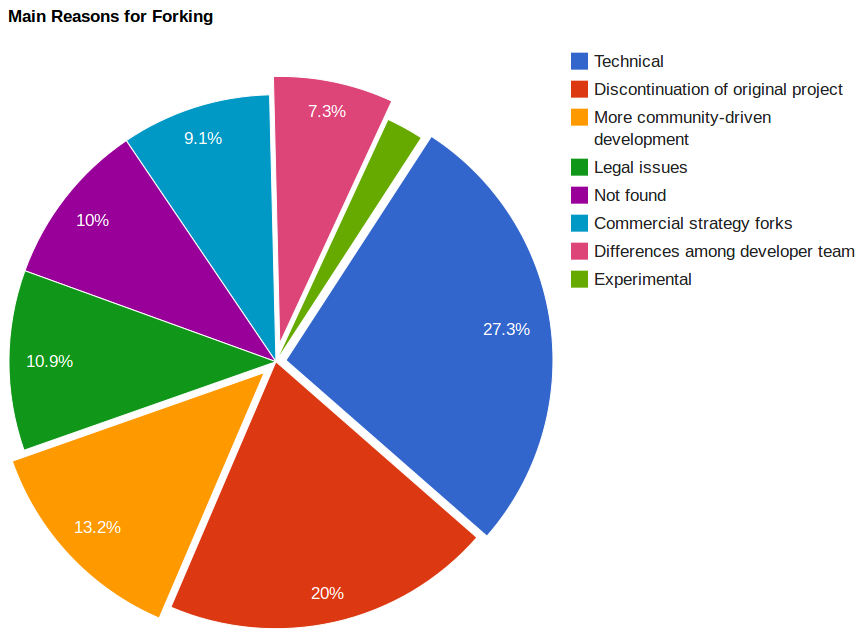
\epsfig{file=ForkingReasonsPieChart.png, width=\columnwidth}
\end{figure}

This proposal report is organized as follows: Section \ref{relatedwork} presents related literature on open source social communities, the gap in the literature, and discusses why the issue needs to be studied. 
Then, Section \ref{ResearchGoals} presents our research objective and research questions. After that, in section \ref{methodology} presents how data gathering, statistical modeling, and qualitative analysis are proposed to be done, as well as our initial hypotheses. In section \ref{sectionInitialStudy}, we present results of our initial study. Section \ref{timelineSection}, shows the proposed timeline for the research and the author's graduation. And lastly, section \ref{threatsToValidity} we discuss the threats to validity.\\
\pagebreak

\section{Related Work}
\label{relatedwork}

The free and open source software development communities have been studied extensively. Researchers have studied the social structure and dynamics of team communications \cite{Bird}\cite{Guzzi}\cite{HowisonSocialDynamics}\cite{HowisonFlossMole}\cite{Nakakoji}, identifying knowledge brokers and associated activities \cite{Sowe}, project sustainability \cite{Nakakoji}\cite{NymanForkingSustainability}, forking \cite{NymanCodeForking}, requirement satisfation \cite{Ernst}, their topology \cite{Bird}, their demographic diversity \cite{Kunegis}, gender differences in the process of joining them \cite{Kuechler}, and the role of age and the core team in their communities \cite{AzarbakhtOSS2014}\cite{AzarbakhtINSNA2014}\cite{DavidsonVLHCC2014}\cite{Torres}. Most of these studies have tended to look at community as a static structure rather than a dynamic process \cite{CrowstonFLOSSWhatWeKnow}. This makes it hard to determine cause and effect, or the exact impact of social changes.

Post-forking porting of new features or bug fixes from peer projects happens among forked projects \cite{Baishakhi}. A case study of the BSD family (i.e., FreeBSD, OpenBSD, and NetBSD, which evolved from the same code base) found that 10-15\% of lines in BSD release patches consist of ported edits, and on average 26-58\% of active developers take part in porting per release. Additionally, They found that over 50\% of ported changes propagate to other projects within three releases \cite{Baishakhi}. This shows the amount of redundant work developers need to do to synchronize and keep up with development in parallel projects. 

Visual exploration of the collaboration networks in FOSS communities was the focus of a study that aimed to observe how key events in the mobile-device industry affected the WebKit collaboration network over its lifetime. \cite{JoseWebKit} They found that \textit{coopetition} (both competition and collaboration) exists in the open source community; moreover, they observed that the ``firms that played a more central role in the WebKit project such as Google, Apple and Samsung were by 2013 the leaders of the mobile-devices industry. Whereas more peripheral firms such as RIM and Nokia lost market-share'' \cite{JoseWebKit}. 

The study of communities has grown in popularity in part thanks to advances in social network analysis.  From the earliest works by Zachary \cite{Zachary} to the more recent works of Leskovec et al. \cite{LeskovecGraphsOverTime}\cite{LeskovecStatisticalPropertiesOfCommunityStructure}, there is a growing body of quantitative research on online communities. The earliest works on communities was done with a focus on information diffusion in a community \cite{Zachary}. The study by Zachary investigated the fission of a community; the process of communities splitting into two or more parts. They found that fission could be predicted by applying the Ford-Fulkerson min-cut algorithm \cite{Ford} on the group's communication graph; ``the unequal flow of sentiments across the ties'' and discriminatory sharing of information lead to subcommunities with more internal stability than the community as a whole.\cite{Zachary}

The dynamic behavior of a network and identifying key events was the aim of a study by Asur et al \cite{Asur}. They studied three DBLP co-authorship networks and defined the evolution of these networks as following one of these paths: a) Continue, b) k-Merge, c) k-Split, d) Form, or e) Dissolve. They defined four possible transformation events for individual members: 1) Appear, 2) Disappear, 3) Join, and 4) Leave. They compared groups extracted from consecutive snapshots, based on the size and overlap of every pair of groups. Then, they labeled groups with events, and used these identified events \cite{Asur}.

\begin{table}[!htbp]
\caption{The behavioral measures used by Asur et al. \cite{Asur}}
\label{tableDiversityMeasuresAsurEtAl} 
\begin{tabular}{p{0.2\columnwidth} p{0.7\columnwidth}}
\hline\noalign{\smallskip}
\textbf{Metrics} & \textbf{Meaning} \\
\noalign{\smallskip}\hline\noalign{\smallskip}
Stability & Tendency of a node to have interactions with the same nodes over time \\ \hline
Sociability & Tendency of a node to have different interactions \\\hline
Influence & Number of followers a node has on a network and how its actions are copied and/or followed by other nodes. (e.g., when it joins/leaves a conversation, many other nodes join/leave the conversation, too) \\\hline
Popularity & Number of nodes in a cluster (how crowded a sub-community is) \\
\noalign{\smallskip}\hline
\end{tabular}
\end{table}

The communication patterns of free and open source software developers in a bug repository were examined by Howison et al. \cite{HowisonSocialDynamics}. They calculated out-degree centrality as their metric. Out-degree centrality measures the proportion of times a node contacted other nodes (outgoing) over how many times it was contacted by other nodes (incoming). They calculated this centrality over time ``in 90-day windows, moving the window forward 30 days at a time.'' They found that ``while change at the center of FOSS projects is relatively uncommon,'' participation across the community is highly skewed, following a power-law distribution, where many participants appear for a short period of time, and a very small number of participants are at the center for long periods. Our proposed approach is similar to theirs in how we form collaboration graphs. Our approach is different in terms of our project selection criteria, the metrics we examine, and our research questions.

The tension between diversity and homogeneity in a community was studied by Kunegis et al. \cite{Kunegis}. They defined five network statistics, listed in Table \ref{TableDiversityMeasuresKunegisEtAl}, used to examine the evolution of large-scale networks over time. They found that except for the diameter, all other measures of diversity shrunk as the networks matured over their lifespan. Kunegis et al. \cite{Kunegis} argued that one possible reason could be that the community structure consolidates as projects mature.

\begin{table}
\centering
\caption{The measures of diversity used by Kunegis et al. \cite{Kunegis}}
\label{TableDiversityMeasuresKunegisEtAl}
\begin{tabular}{p{0.3\linewidth} p{0.3\linewidth} p{0.3\linewidth}}
%\begin{tabular}{l l l}
\hline\noalign{\smallskip}
\textbf{Network property} & \textbf{Network is diverse when} & \textbf{Diversity Measures} \\
\noalign{\smallskip}\hline\noalign{\smallskip}
Paths between nodes & Paths are long & Effective diameter \\ \hline
Degrees of nodes  & Degrees are equal & Gini coefficient of the degree distribution \\ \hline
Communities  & Communities have similar sizes & Fractional rank of the adjacency matrix \\ \hline
Random walks  & Random walks have high probability of return & Weighted spectral distribution \\ \hline
Control of nodes  & Nodes are hard to control & Number of driver nodes \\
\noalign{\smallskip}\hline
\end{tabular}
\end{table}

Community dynamics was the focus of a more recent study by Hannemann and Klamma \cite{Hannemann} on three open source bioinformatics communities. They measured "age" of users, as starting from their first activity and found survival rates and two indicators for significant changes in the core of the community. They identified a survival rate pattern of 20-40-90\%, meaning that only 20\% of the newcomers survived after their first year, 40\% of the survivors survived through the second year, and 90\% of the remaining ones, survived over the next years. As for the change in the core, they suggested that a falling maximum betweenness in combination with an increasing network diameter as an indicator for a significant change in the core, e.g., retirement of a central person in the community. Our initial network-specific study built on their findings, and the evolution of betweenness centralities and network diameters for the projects in our study are explained in the following sections.
\pagebreak

\section{Research Goals}
\label{ResearchGoals}

Social interactions reflect the changes the community goes through, and so, it can be used to describe the context surrounding a forking event. Social interactions in FOSS can happen, for example, in the form of mailing list email correspondence, bug report issue follow-ups, and source code co-authoring. At least, three of the seven main reasons for forking \cite{Robles}, as listed in Table \ref{tableReasonsForForking} and Figure \ref{tableReasonsForForking} are socially related, and so, their effects should be reflected in the developers' interactions data. These three reasons are (1) Personal differences among developer team, (2) The need for more community-driven development, and (3) Technical differences for addition of functionality. Given the data, these are the three categories that may be identified using longitudinal modeling of the interactions, without digging into the contents of the communications. The other categories could be the focus of another research study, whose scope does not have a large overlap with the scope of this study. \\
As an example, if a fork occurred because of a desire for ``more community-driven development'', we expect to see interaction patterns in the collaboration data showing a strongly-connected core that is hard to penetrate for the rest of the community. In other words, in this case, the power stays in the hands of the same people throughout, as new people come and go. 

In this study, we plan to analyze, quantify and visualize how the community is structured, how it evolves, and the degree to which community involvement changes over time.
Specifically, our research objectives and research questions are listed in the following subsections \ref{ResearchObjective} and \ref{RQs}.

\subsection{Research Objectives}
\label{ResearchObjective}
\subsection*{What are the social patterns associated with different types of undesirable forking?\\}

\subsubsection{\hspace{4 mm} Do forks leave traces in the collaboration artifacts of open source projects in the period leading up to the fork?\\}

To study the properties of possible social patterns, we need to verify their existence. More specifically, we need to check whether the possible social patterns are manifested in the the collaboration artifacts of open source projects, e.g., mailing list data, issue tracking systems data, source code data. This is going to be accomplished by statistical modeling of developer interactions as explained in more detail in section \ref{methodology}.

\subsubsection{\hspace{4 mm} Do different types of forks leave different types of traces?\\}

If forks leave traces in the collaboration artifacts, do forks exhibit different social patterns? Are there patterns that exemplify these categories? For example, is there a prototypical ``personal differences'' fork collaboration pattern? If so, do different forking reasons have distinctly different social patterns associated with them? Is a project labeled as a ``technical differences'' fork only a ``technical differences'' fork? Or, alternatively, can they be a mix of several reason categories?

We are going to investigate this by statistical modeling of the interaction graphs, as explained in detail in section \ref{statisticalModel}.

\subsubsection{\hspace{4 mm} What are the key indicators that let us distinguish between different types of forks?\\}

What quantitative measure(s) can be used as an early warning sign of an inflection point (fork)? Are there metrics that can be used to monitor the odds of change, (e.g. forking-related patterns), ahead of time? This will be accomplished by statistical modeling of developer interactions as explained in more detail in section \ref{methodology}.

%\subsubsection*{R.Q. 4 \hspace{4 mm} Does our analysis match what people in the community remember?\\} 
%
%To validate what our quantitative data mining approach finds, we can compare it to what people remember of the situation, and what is written about that project. This validation check requires interviewing people from the studied forked projects. Semi-structured interviews need to be conducted, with as many developers from the forked projects, till the interviewers reach a point of saturation (i.e., when no new information is gained by doing more interviews). These semi-structured interviews will be recorded, transcribed, and open-coded, to find common patterns in the interviewees responses.
%

%To complement the study, a literature review and web research will be done to gather data that was written about the project, before the fork and after the fork dates. The content of the messages send and received by the top contributors of the project in the month leading to the forking events can be a read and analyzed to complement the findings of the interview study. 
\pagebreak

\section{Methodology}
\label{methodology}

Detecting change patterns, requires gathering  relevant data, cleaning it, and analyzing it. In the following subsections, we describe the proposed process in detail. 

\subsection{Phase 1: Data Collection}
\label{DataCollection}

\subsubsection{The Case of Undesirable forking}
To find patterns uniquely associated with undesirable forks, we need to gather data on projects from the following three categories: 

\begin{table} [H]
\caption[Undesirable forking vs. Other categories]{The three types of projects for which data is collected in this study}
\label{tableUndesirableForkingDataCollect} 
\begin{tabular}{p{0.7\columnwidth} p{0.2\columnwidth}}
\hline\noalign{\smallskip}
\textbf{Type of forking} & \textbf{Abbreviation} \\
\noalign{\smallskip}\hline\noalign{\smallskip}
Undesirable \& socially-related forking & U.F. \\ \hline
Other (Healthy/Other) \& socially-related forking & H.F. \\\hline
No forking at all & No.F. \\
\noalign{\smallskip}\hline
\end{tabular}
\end{table}

We define Undesirable Forking (U.F.) as the projects forked because of \textit{Personal differences among developers team}, or because of the need for \textit{more community-driven development}. One-fifth (20.5\%) of the 220 forked projects fall into this category.

Other (Healthy/Other) (H.F.) is defined as projects forked because of \textit{technical differences (Addition of functionality)}. More than a quarter (27.3\%) of the 220 forked projects fall into this category.

These three categories are the socially-related categories, which means, the social context during the run-up to forking arguably should be reflected in their social interactions. 

To find projects in U.F. and H.F. categories, we looked at the list of all significant open source software forks in the past three decades as compiled by Robles and Gonzalez-Barahona \cite{Robles}. They found the reasons behind each fork, listed in Table \ref{tableReasonsForForking}. We applied three selection criteria to the 220 forked projects on that list to find projects in U.F. and H.F. categories. A project was short-listed as either a U.F. or H.F. if \textbf{a)} the forking was recent, i.e., happened after the year 2000, \textbf{b)} its data was existent and available to access and download online, or was made accessible to us after our requests; and \textbf{c)} the project had a sizable developer community, i.e., more than a dozen developers, which means it would be large enough to make a sociogram for a meaningful statistical analysis. For the No.F. category, we chose well-known, stable projects that have been active long enough (to experience turbulence; defined as two years); and yet have not forked; and are similar in size of the development team. Similarity in size is a constrain that our statistical method imposes for the results to be meaningful, as described in detail in section \ref{statisticalModel}.  The preceding criteria resulted in the projects listed in Table \ref{forkedProjectsDataCollected}. The rest of the 220 forked projects were discarded, because they did not meet the described filtering criteria.


\begin{table}
\centering
\caption{List of projects in U.F. H.F., and No.F. categories selected based on the criteria described in section \ref{DataCollection} for our study}
\label{forkedProjectsDataCollected}
\begin{tabular}{p{0.39\textwidth} p{0.48\textwidth} p{0.135\textwidth} p{0.07\textwidth}}
\hline\noalign{\smallskip}
\textbf{Projects} & \textbf{Reason for forking} & \textbf{Year forked} & \textbf{Type}\\
\noalign{\smallskip}\hline\noalign{\smallskip}
Kamailio \& OpenSIPS & Differences among developer team & 2008 & U.F.\\ \hline
ffmpeg \& libav & Differences among developer team & 2011 & U.F.\\ \hline
Asterisk \& Callweaver & More community-driven development & 2007 & U.F.\\ \hline
rdesktop \& FreeRDP  & More community-driven development & 2010 & U.F.\\ \hline
freeglut \& OpenGLUT & More community-driven development & 2004 & U.F.\\ \hline
Amarok \& Clementine Player & Technical (Addition of functionality) & 2010 & H.F.\\ \hline
Apache CouchDB \& BigCouch & Technical (Addition of functionality) & 2010 & H.F.\\ \hline
Pidgin \& Carrier & Technical (Addition of functionality) & 2008 & H.F.\\ \hline
MPlayer \& MPlayerXP & Technical (Addition of functionality) & 2005 & H.F.\\ \hline
Ceph  & Not forked & - & No.F.\\ \hline
Python & Not forked & - & No.F.\\ \hline
OpenStack Neutron & Not forked & - & No.F.\\ \hline
GlusterFS & Not forked & - & No.F.\\ 
\noalign{\smallskip}\hline
\end{tabular}
\end{table}

\subsubsection{Data Sources}
The data sources to collect are \textbf{a)} developer mailing lists, where developers' interact by sending and receiving emails, \textbf{b)} Issue(bug) tracking systems, where developers interact by reporting an issue/bug, discussing how to resolve it, and closing the issues, and , \textbf{c)} Source-code repository contribution logs, where developers interact by modifying the code, and/or working on the same source files. The sociograms will be formed based on interactions among developers in any of the preceding data sources. 
% \textbf{d)} (Proposed) The content of the messages send and received by the top contributors of the project in the months leading to the forking events can be a good data source to be sentiment-analyzed. Using sentiment analysis, we can quantify the level of positive/negative language usage, and may detect events, for example, in-fighting where people involved in the conflict exchange negative sentiments.

The time period for which data was collected is one year leading to when the fork happened. This should supposedly capture the social context prior, and at the time of the fork.

\subsection{Phase 2: Sociogram Formation and Statistical Study}

Social connections and non-connections can be represented as graphs, in which the nodes represent actors and the edges represent the interaction(s) between actors or lack thereof. Such graphs can be a snapshot of a network -- a static sociogram -- or a changing network, also called a dynamic sociogram. In this phase, we process interactions data to form a communication sociogram of the community. Two types of analysis can be done on sociograms; \textbf{a)} a \textit{cross-sectional} study, and \textbf{b)} a \textit{longitudinal} study. We are interested in patterns in the run-up to forks, so, we choose to do a longitudinal study, unlike most existing research on forking. This is a novel contribution of our study.

A longitudinal study can look at the sociograms in two distinct approaches: \textbf{a)} a \textit{network-specific} approach, in which, we focus on the actual networks under study, to describe the structure of the \textit{observed networks} with numeric summaries/descriptors to describe the structure and what we actually see, e.g., in Figures \ref{figureNodesEdgesTimeR} and \ref{figureDiameterTimeR}. Or, \textbf{b)} a \textit{population-processes} approach, in which, we treat the observed network as one realization from a set of all possible networks with the same number of nodes, and with similar characteristics. To this end, the observed network, is only good to help us understand the social forces/processes that generated it.

Figures \ref{figureNodesEdgesTimeR} and \ref{figureDiameterTimeR} are good examples of the expressiveness as well as the limitation of a network-specific approach. Figure \ref{figureNodesEdgesTimeR} shows the normalized change in the number of active nodes (developers) and edges (interaction between developers) for eight FOSS projects from U.F. and H.F. categories. The normalized number of nodes and edges for the U.F. forks (i.e., second and third row) show a sudden sharp decrease around the month of fork. This can be because of dissolution of the development team, who either left the project, or stopped being active contributors as much as before. Figure  \ref{figureDiameterTimeR} shows normalized change of diameter over time for the same projects. It is hard to make sense of normalized diameter changes across projects, and this demonstrates the limitations of network-specific approaches, as they may, or may not (often the case), help us understand the network dynamics.

The following subsection lists the reasons why we need to use a statistical model, used in the \textit{population-processes approach}.

\subsubsection{Why a statistical model is needed?}
One may wonder why we should look beyond the observed network. We can do measurements on the observed networks data, and get some descriptive statistics. This would be a superficial look at the data, and even though necessary, is not good enough and has several shortcomings. 
There is another way of looking at these networks, in a less-superficial way; namely, finding a model that fits the data and its longitudinal change. So, instead of a superficial look at the data, we can find a well-fitting statistical model of our observed interactions network. The following lists the reasons why we need to go beyond a superficial measurement-only approach. 

\begin{enumerate}

\item For the \textit{observed network}, a small observation error or sampling error, and the uncertainty involved with real-world communication, can result in large perturbation in the numeric descriptors used to describe static graphs. 

\item The traditional \textit{network-specific} approach assumes edges in sociograms are statistically independent, (and/or identically distributed). This can be misleading, as, social network data are relational. For example, in real-life human communication, the likelihood of forming ties with friends of a friend is higher than a stranger, as Balance Theory suggests \cite{Heider}. 

\item In population-specific approach, we try to identify the social forces that have formed the observed network, by simulation a population of similar networks of the same characteristics. After finding the statistical distribution of network population, then we can compare the observed network to the population distribution of possible networks of that size, and see how significant and likely it is to observe such a graph, as compared to observing a randomly-generated graph. This is useful, because it gives us a reference point to compare our observed graph with, and to weed out the properties generated by random processes, and to find the statistically significant network statistics. In short, with a statistical model, we can draw inferences about whether certain network structures and substructures are more commonly observed in the observed network than might be expected by chance \cite{Robins}. 

\item Stochastic models capture the regularities in the processes that caused the network ties form, as well as variability that are hard to model otherwise. A model that considers stochasticity allows us to understand the uncertainty associated with an observed network. It makes it possible to learn about the distribution of possible networks for a given specification of a model \cite{Robins}.

\item Different social processes may manifest similar network structures. For example, clustering in a network might be because of structural effects, e.g., structural balance, or through node-level effects, e.g., homophily. To determine which one is the case in our observed network, a statistical model that incorporates both covariates can help. We then can assess the contribution of each covariate, and infer which social process underlies the observed network \cite{Robins}. 

\item  Localized processes might not scale to the entire network well. The combination of the overall structure and the localized processes is hard to investigate without a model. (This micro-macro difference may be investigated through model simulation.)\cite{Robins}

\end{enumerate}

In summary, a measurement-only approach would not be able to explain the longitudinal changes in an open source community's network properly. It can confuse us, and it can mislead us. Our initial study, described in section \ref{results}, is an example of a measurement-only approach, which shows such limitations. This initial study guided in the proper direction; namely, trying to find a statistical model that can explain the networks' longitudinal changes. In the following section \ref{statisticalModel}, we described such a model.  


%\textbf{2)} \textbf{Signaling theory}, from evolutionary biology, and economics \cite{Spence}, tries to explain communication between individuals, in terms of signals. As an example, a person in a community will help others who are in need, if helping signals the helper's desirable personality. This signal helps in attracting mates and results in higher reproduction of that person. In this scenario, the cost of helping another person is less than the benefit gained by the person because of signaling their conditions. 
%
%We may explain the increase of decrease in preferential attachment in U.F. projects, as a result of software developers signaling others in the community of their status, by helping others in need (i.e., peripheral community members), which in turn brings them social prestige.

\subsection{The Statistical Model}
\label{statisticalModel}

Longitudinal evolution of a network data is the result of many small atomic changes occurring between the the consecutively observed networks. In our case, software developers are the actors in the networks, and they can form a connection with another actor, break off an existing connection, or maintain their status quo. These are the four possibilities of atomic change within our evolving networks: (1) forming a new tie; (2) breaking off an existing tie; (3) maintaining a non-connection; and (4) maintaining a connection. We assume a continuous-time network evolution, even though our observations are made at two or more discrete time points. 

The state-of-the-art in studying longitudinal social networks, is the idea of \textit{actor-oriented models} \cite{Snijders2010}, based on a model of actors changing their outgoing ties as a consequence of a stochastic optimization of an \textit{objective function}. This framework assumes that the observed networks at discrete times, are outcomes of a continuous-time Markov process. In the case of open source developers, the actor-oriented model, can be informally described as OpenSourceDeveloper-oriented model, in which, it is assumed that developers are in charge of their communication and collaboration choices. They choose to have interactions with certain other developers and/or they choose to stop having interactions with another developer. In short, they have autonomy in choosing their connections.

Let the data for our statistical actor-oriented model be $M$ repeated observations on a network with \textit{g} actors. The $M$ observed networks (at least two) are represented as directed graphs with adjacency matrices $X(t_m) = (X_{ij}(t_m)))$ for $m = 1,...,M$, where $i$ and $j$ range from a to $g$. The variable $X_{ij}$ shows whether at time $t$ there exists a tie from $i$ to $j$ (value 1) or not (value 0). Be definition, $\forall i, X_{ii}=0$ (i.e. the diagonal of the adjacency matrices).

In order to model the network evolution from $X(t_1)$ to $X(t_2)$, and so on, it is natural to treat the network dynamics as the result of a series of small atomic changes, and not bound to the observation moment, but rather as a more of less continuous process. In this way, the current network structure is a determinant of the likelihood of the changes that might happen next \cite{Coleman1964}. 

For each change, the model focuses on the actor whose tie is changing. We assume that actor $i$ has control over the set of outgoing  tie variables $(X_{i1}, ..., X_{ig})$ (i.e. the $i^{th}$ row of the adjacency matrix). The network changes one tie at a time. We call such an atomic change a \textit{ministep}. The moment at which actor $i$ changes of of his ties, and the kind of change that he makes, can depend on attributes represented by observed covariates, and the network structure. The moment is stochastically determined by the \textit{rate function}, and the particular change to make, is determined by the \textit{objective function} and the \textit{gratification function}. These three functions and their definitions taken from \cite{Snijders2004} are explained in detail the following subsections.

\subsubsection{Rate Function}

The rate function for a developer is the rate at which that developer's outgoing connections changes occur. Or, more formally, we can say, the \textit{rate function} $\lambda_i(x)$ for actor $i$ is the rate at which in actor $i$'s outgoing ties changes occur. It models how frequently the actors make ministeps.\\
The rate function is formally defined \cite{Snijders2004} by
\begin{equation}
\lambda_i(x) = \lim_{dt \to 0} \frac{1}{dt} \mathrm {P} \big({X_{ij}(t + dt) \neq X_{ij}(t) \quad for \quad some \quad j \in \{i, ..., g\} | X(t) = x)}\big).
\end{equation}

The simplest specification of the rate of change is that all actors have the same rate of change of their ties. 

\subsubsection{Objective Function}

The \textit{objective function} $f_i(s)$ for actor $i$ is the value attached to the network configuration $x$. 

The idea is that, given the opportunity to make a change in his outgoing tie variables $(X_{i1},...,X_{ig})$, actor $i$ selects the change that gives the greatest increase in the objective function. We assume that if there is difference between actors in their objective functions, these differences can be represented based on the model covariates \cite{Snijders2004}. 

Let's denote the present network by $x = X(t)$. The new network that would be the result of a ministep (i.e. changing a single tie variable $x_{ij}$ into its opposite $1 - x_{ij}$ ) by actor $i$ is denoted by $x(i \mapsto j)$. This choice is modeled in the following way: 

Let $U(j)$ denote a random variable which represents the attraction for $i$ to $j$. We assume that these $U_j$ are random variables distributed symmetrically about 0, and independently generated for each new ministep. In this way, the actor $i$ chooses to change his tie variable with the other actor $j$ for whom the following value \cite{Snijders2004} is the highest:

\begin{equation}
f_i(x(i \mapsto j)) + U(j)
\end{equation} 

This is a myopic stochastic optimization rule: myopic because only the situation one step after the current step is considered; and stochastic because the unexplained part is modeled by a random variable $U(j)$. 

$U(j)$ is chosen to have Gumbel distribution with mean 0 and scale parameter 1. In this way, the probability that actor $i$ chooses to change $x_{ij}$ for any particular $j$, given that such a change happens, is \cite{Snijders2004},

\begin{equation}
p_{ij}(x) = \frac{exp(f_i(i \mapsto j) - f_i(x))}{\sum_{h=1, h \neq i}^{g} exp(f_i(i \mapsto h) - f_i(x))}
\end{equation}

\subsubsection{Gratification Function}
Sometimes the order in which changes occur makes a difference for the desirability of the network. Such differences cannot be represented by the objective function. So, we need another function, called gratification function. \\

The \textit{gratification function} $g_i(x,j)$ for actor $i$ is the value attached to this actor (in addition to what follows from the objective function) to the act of changing the tie variable $x_{ij}$ from $i$ to $j$, given the current network configuration $x$. 

In the case that a gratification function is included, the actor $i$ chooses to change $x_{ij}$ for that other actor $j$ for whom the following value \cite{Snijders2004} is the highest:

\begin{equation}
f_i(x(i \mapsto j)) + g_i(x, j) + U(j)
\end{equation} 

And we will have 
\begin{equation}
\label{ObjectiveFunctionWithGratification}
p_{ij}(x) = \frac{exp(f_i(i \mapsto j) + g_i(x, j) - f_i(x))}{\sum_{h=1, h \neq i}^{g} exp(f_i(i \mapsto h) + g_i(x, j) - f_i(x))}
\end{equation}

\subsubsection{Markov Chain Transition Rate Matrix}
The components of the actor-oriented model, described above, define a continuous-time Markov chain on the space $\chi$ of all directed graphs on this set of $g$ actors. 

The transition rate matrix (also called intensity matrix), for this model is given by
\begin{multline}
\label{intensityMatrix}
q_{ij}(x) = \lim_{dt \to 0} \frac{1}{dt} \mathrm {P} \big({X(t + dt) = X(i \mapsto j) | X(t) = x)}\big) \\ = \lambda_i(x) p_{ij}(x)
\end{multline}

Expression (\ref{intensityMatrix}) shows the rate at which actor $i$ makes ministeps, multiplied by the probability that he changes the arc variable $X_{ij}$, if he makes a ministep.\\

\subsubsection{Markov Chain Simulation}
\label{MarkovChainSimulationSteps}
Our Markov chain can be simulated by repeating the following steps \cite{Snijders2004}:

Start at time $t$ with directed graph $x$. 
\begin{enumerate}
\item Define $\lambda_{+} = \sum_{i=1}^g \lambda_i(x)$ and let $\Delta t$ be a random variable with the exponential distribution with parameter $\lambda_{+}(x)$.
\item The actor $i$ is chosen randomly with probabilities $\frac{\lambda_{i}(x)}{\lambda_{+}(x)}$
\item Given this $i$, choose actor $j$ randomly with probabilities 
\begin{equation}
p_{ij}(x) = \frac{exp(f_i(i \mapsto j) + g_i(x, j) - f_i(x))}{\sum_{h=1, h \neq i}^{g} exp(f_i(i \mapsto h) + g_i(x, j) - f_i(x))} \nonumber
\end{equation}
\item Now change $t$ to $t + \Delta t$ and change $x_{ij}$ to $(1 - x_{ij})$
\end{enumerate}

\subsection{Model Specification}
The functions described above need to be supplied with a specific model for the rate, objective and gratification functions. These functions depend on unknown parameters that need to be estimated based on the data. In the following, we explain what functions can be included in these functions.

\subsubsection{Objective Function}
The following weighted sum represents the objective function:

\begin{equation}
f_i(\beta, x) = \sum_{k = 1}^{L} \beta_k s_{ik}(x)
\end{equation}

Parameters $\beta = (\beta_1, ..., \beta_L)$ is to be estimated. Functions $s_{ik}(x)$ can be the following \cite{Snijders2004}:

\paragraph{Structural Effects}
\begin{enumerate}
\item{The reciprocity effect}
\item{The closure effect}

For example, 
\begin{enumerate}
\item Transitive triplets effect. 
\item Transitive ties.
\item Balance
\item Number of actors at distance two
\end{enumerate}
\item{Three-cycles}
\item{Betweenness}
represents brokerage
\item{Density}
\item{Activity}
\item{Actor-oriented covariate V-related popularity}
\item{Actor-oriented covariate V-related activity}
\item{Actor-oriented covariate V-related dissimilarity}
\item{in-in degree assortativity}
\item{in-out degree assortativity}
\item{out-in degree assortativity}
\item{out-out degree assortativity}
\end{enumerate}

\paragraph{Behavior-related Effects\\}
Let's denote a dependent behavior variable as $Z$.
\begin{enumerate}
\item{Shape effect: Explains the drive toward high values on Z}

\item{Quadratic Shape Effect}
\item{Similarity}
\begin{enumerate}
\item{average similarity}
\item{total similarity}
\end{enumerate}
\item{average alter effect}
\end{enumerate}

\subsubsection{Gratification Function}
The following weighted sum represents the gratification function:

\begin{equation}
g_i(\gamma, x, j) = \sum_{h = 1}^{H} \gamma_h r_{ijh}(x)
\end{equation}

Some possibile functions $r_{ijh}(x)$ are the following \cite{Snijders2004}:
\begin{enumerate}
\item Breaking off a reciprocated tie:\\ 
$r_{ij1}(x) = x_{ij} x_{ji}$
\item Number of indirected links for creating a new tie:\\ $r_{ij2}(x) = (1 - x_{ij}) \sum_h x_{ih} x_{hj}$
\item Effect of dyadic covariate W on breaking off a tie:\\
$r_{ij3}(x) = x_{ij}w_{ij}$
\end{enumerate}

\subsection{Markov Chain Monte Carlo (MCMC) Estimation}
The described statistical model for longitudinal analysis of open source software development communities is a complex model and it is not possible to calculate exactly. However, we can simulate the longitudinal evolution, and estimate the model based on the simulations. Then we can choose an estimated model that has a good fit to the network data.
The following section described the simulation and estimation procedures. 


Network evolution can be simulated using a MCMC estimation method. The method of moments (MoM) can be used in the following way \cite{Snijders2004}: \\

Let $x^{obs}(t_m), m = 1, ..., M$ be the observed networks, and the objective function be $f_i(\beta, x) = \sum_{k=1}^L \beta_k s_{ik}(x)$. 
In MoM, the goal is to determine the parameters $\beta_k$ such that, summed over $i$ and $m$, the expected values of the $s_{ik}(X(t_{m+1}))$ are equal to the observed values. In other words, MoM fits the \textit{observed} to the \textit{expected}. 
The observed target values are:
\begin{equation}
s_k^{obs} = \sum_{m=1}^{M-1}\sum_{i=1}^g s_{ik}(x^{obs}(t_{m+1})) \quad (k = 1, ..., L)
\end{equation}

The simulations run as follows \cite{Snijders2004}:
\begin{enumerate}
\item The distance between two directed graphs $x$ and $y$ is defined as
\begin{equation}
\norm{x -y} = \sum_{i,j}\abs{x_{ij} - y_{ij}}
\end{equation}
and let the observed distances for m = 1, ..., M-1 be 
\begin{equation}
c_m = \norm{x^{obs}(t_{m+1})-x^{obs}(t_m)}
\end{equation}
\item Use the $\beta$ parameter vector and the rate of change $\lambda_{i}(x) = 1$

\item Do the following for m = 1, ..., M-1
\begin{enumerate}
\item Define the time as 0, and start with $X_m(0) = x^{obs}(t_m)$
\item Simulate the model, as described in \ref{MarkovChainSimulationSteps} until the first time point, where 
\begin{equation}
\norm{X_m(R_m) - x^{obs}(t_m)} = c_m
\end{equation}
\end{enumerate}
\item For k = 1, ..., L, calculate the following statistics:
\begin{equation}
S_k = \sum_{m = 1}^{M-1}\sum_{i=1}^{g}s_{ik}(X_m(R_m))
\end{equation}
\end{enumerate}

The simulation output will be the random variables $(S,R) = (S_1,...,S_L,R_1,...,R_{M-1})$. The desirable outcome for the estimation is the vector parameter $\hat{\beta}$ for which the expected and the observed vectors are the same. 
% $\mathcal{E}_{\hat{\beta}}S = s^{obs}$.

\subsection{Hypothesis Testing}
So far, we have described what we can model, how to fit a model that explains the longitudinal changes in an open source community (or any similar network). Now, we can test several hypothesis about these models. For example, we can test whether a particular effect's (for example, reciprocity's) statistical significance on the model, and make meaningful statements about whether the network dynamics depends on this parameter with a p-value, indicating the significance level. Such test is explained in section \ref{singleParameterTest}.

Or, alternatively, we can compare two models for two open source project communities, and make statements about the difference in several model effects, for example, reciprocity and three-cycles, using the method described in section \ref{multiParameterTest}. 

Or, lastly, we may compare several open source communities (or such networks) and test the statistical significance of the differences between their models, using the methods described in section \ref{MANOVA}. This allows us to compare within-group and across-group comparisons of longitudinal models of open-source projects. In this study, we do all three discussed forms of tests of significance. In the following subsections, the details of these tests are described.   


\subsubsection{Single Parameter Test}
\label{singleParameterTest}
Using the actor-oriented model, t-type test of single parameters can be done using the parameter estimates and their standard errors (S.E.). 
For example, for testing the null hypothesis that a component $k$ of the parameter vector $\beta$ is 0, the test has approximately a standard normal distribution. For this null hypothesis: 
\begin{equation}
H_0: \beta_k = 0;
\end{equation}
the t-test can be done using the following t-statistic:
\begin{equation}
\frac{\hat{\beta_k}}{S.E.(\hat{\beta_k})}
\end{equation}
Given a p-value $\leq$ 0.05 would indicate a strong evidence that the network dynamics depends on the corresponding parameter's effect. 

\subsubsection{Multi-Parameter Differences Between Groups}
\label{multiParameterTest}
Given the parameter estimates $\hat{\beta_a}$ and $\hat{\beta_b}$, and their standard errors $S.E._a$ and $S.E._b$, the differences between two groups can be tested using the following t-statistics. This t-statistics, under the null hypothesis of equal parameters, has an approximately standard normal distribution:
\begin{equation}
\frac{\hat{\beta_a}-\hat{\beta_b}}{\sqrt{S.E._a^2 + S.E._b^2}}
\end{equation}

\subsubsection{Multivariate Analysis of Variance Between Multiple Groups}
\label{MANOVA}
To test the statistical significance of the mean differences between groups (in our case, the different categories of forking), we may use Multivariate Analysis of Variance (MANOVA) method. In contrast to ANOVA, MANOVA method tests for the difference in two or more vectors of means. 

\subsection{Research Questions and Hypotheses}
\label{RQs}
In section \ref{ResearchObjective}, we described the research objectives in general terms. Now that we have described how to model the longitudinal changes in an open source community's collaboration networks, we can be more specific about the research questions, and the hypotheses for our statistical tests. The following are the null hypotheses for across-group comparisons using the Multivariate Analysis of Variance Between Multiple Groups tests.

\subsubsection{Null Hypothesis \# 1:} 
There are no statistically significant differences in vectors of means of the actor-oriented model of longitudinal changes of software projects in U.F. category and No.F. category.

\subsubsection{Null Hypothesis \# 2:} 
There are no statistically significant differences in vectors of means of the actor-oriented model of longitudinal changes of software projects in H.F. category and No.F. category.

\subsubsection{Null Hypothesis \# 3:} 
There are no statistically significant differences in vectors of means of the actor-oriented model of longitudinal changes of software projects in U.F. category and H.F. category.


\subsection{Predictions}
Software development is a collective effort, and software developers are human beings, so, theories about human behavior from sociology and psychology could help explain how software developers interact and collectively develop software. In particular, the following theories about human behavior are the bases for our hypotheses. They complement each other in term of explaining the context of forking.

\subsubsection{Behavior Models}
\paragraph{} \textbf{Balance theory} \cite{Heider} talks about a motivation of individuals to move toward psychological balance. Balance theory considers cognitive consistency as a motive that drives sentiment or liking relationships, as well as liking of things created by or associated with the alter in the relationship.

We may explain U.F. forked projects because of ``personal differences'' as a results of cognitive inconsistency between the liking relationship of other developer(s) and the software and community created by or associated with them. 

\paragraph{} \textbf{Assortativity theories}, which tries to explain collaboration, and people's preference for interacting with others who are similar to them in some way. This is related to reciprocity, in forms of contingent, direct, and indirect reciprocity. Homophily and Heterophily, which affect diversity of networks, are also closely related to assortative selection.

We may explain U.F. forked projects because of ``more community-driven development'' as a by-result of developers' homophile collaborator selection.



% %%%%%%%%%%%%%%%%%%%%%%%%%%%%%%%%%%%%%%%%%%%%%%%%%%%%%%%
% %%%%%%%%%%%%%%%%%%%%%%%%%%%%%%%%%%%%%%%%%%%%%%%%%%%%%%%
%A recent method for population-process approach is exponential family random graph models (ERGM) \cite{Robins}, in which, the possible edges between nodes of a graph are regarded as random variables. Assumptions about dependencies among these random variables determine the form of the ERGM model for the network. The model parameters are estimated using the observed network, which in turn, can be used to interpret the underlying processes that generated the observed network. For example, we can infer whether a model parameter's effect is significant, and hence, whether the characteristic seen in the observed network is more or less likely than expected by chance.
%
%The general form of the exponential family random graph models is \cite{Krivitsky}: 
%
%\begin{equation} P(Y=y)=\frac{\exp(\theta'g(y))}{k(\theta)} \end{equation}
%where:
%\begin{itemize}
%\item Y is the random variable for the state of the network,
%\item \( g(y) \) is the vector of model statistics for network y,
%\item \( \theta \) is the vector of coefficients for model statistics, 
%\item \( k(\theta) \) represents the quantity in the numerator summed over all possible networks with the same node set as y \cite{Krivitsky}.
%\end{itemize}
%This can be written in terms of the conditional log-odds of a single actor pair \cite{Krivitsky}:
%
%\begin{equation} \operatorname{logit}{(Y_{ij}=1|y^{c}_{ij})=\theta'\delta(y_{ij})} \end{equation}
%where: 
%\begin{itemize}
%\item \( Y_{ij} \) is the random variable for the state of the actor pair \( i,j \) (with realization \( y_{ij} \)), 
%\item \( y^{c}_{ij} \) signifies the complement of \( y_{ij} \), i.e., all dyads in the network other than \( y_{ij} \). 
%\item \( \delta(y_{ij}) \) equals \( g(y^{+}_{ij})-g(y^{-}_{ij}) \), where 
%\item \( y^{+}_{ij} \) is defined as \( y^{c}_{ij} \) along with \( y_{ij} \) set to 1,
%\item \( y^{-}_{ij} \) is defined as \( y^{c}_{ij} \) along with \( y_{ij} \) set to 0.
%\item That is, \( \delta(y_{ij}) \) equals the value of \( g(y) \) when \( y_{ij}=1 \) minus the value of \( g(y) \) when \( y_{ij}=0 \), but all other dyads are as in \( g(y) \). This emphasizes the log-odds of an individual tie conditional on all others. 
%\item \( g(y) \) is called the \textit{statistics} of the model, and \(\delta(y_{ij}) \) the ``\textit{change statistics}'' for actor pair \( y_{ij} \) \cite{Krivitsky}.
%\end{itemize}
%
%The model parameters are usually estimated using a pseudo-likelihood estimation (PLE) method or Markov chain Monte Carlo maximum likelihood estimation (MCMCMLE) \cite{SnijdersMCMCMLE}. 
%
%As in the case of our longitudinal study of dynamic networks, we need to use an extension of ERGMs, namely, Separable Temporal Exponential Family Random Graph Models (STERGM), which takes two models, one for the formation, and another for dissolution \cite{Krivitsky}.
%
%
%\begin{table*}
%\centering
%\caption{Summary of expectations for the statistical model covariates, and sentiment analysis for each forking category. An expected ``no significant change'' is denoted by a dash ($-$) line.}
%\label{tabelSummaryExpectationModelParameters}       
%\begin{tabular}{m{0.4\columnwidth} m{0.15\columnwidth} m{0.15\columnwidth} m{0.15\columnwidth} m{0.15\columnwidth}}
%\hline\noalign{\smallskip}
%\textbf{Model parameter} & \textbf{U.F. Pers. Dif.} & \textbf{U.F. More Comm.} & \textbf{H.F. Tech. Dif.} & \textbf{No.F.}\\
%\noalign{\smallskip}\hline\noalign{\smallskip}
%Outdegree & - & - & - & - \\ \hline
%Reciprocity & decrease & - & - & - \\ \hline
%Balance & - & - & - & - \\ \hline
%3-cycle & decrease & decrease & - & - \\ \hline
%Transitive triplets & - & - & - & - \\ \hline
%Transitive ties & - & - & - & - \\ \hline
%Betweenness & increase & - & increase & - \\ \hline
%Clustering Coefficient & - & - & - & - \\ \hline
%Preferential Attachment & - & - & - & - \\ \hline
%Assortativity & - & increase & - & - \\
%%CUSUM betweenness & sharp increase & - & increase & - \\ \hline
%%Sentiment Analysis & increase in negativity & - & - & - \\
%\noalign{\smallskip}\hline
%\end{tabular}
%\end{table*}
%
%\subsubsection{Model Covariates}
%\label{modelCovariates}
%What covariates to include depends on the context, and the data available for developers.
%Table \ref{tableCovariates} lists several explanatory variables that can be included for modeling the community evolution. Table \ref{tabelSummaryExpectationModelParameters} lists what we expect to see associated with different types of forking. Specifically, for each of the following forking categories, we expect the following model parameters:
%
%For ``personal differences'' forks (U.F.), we expect to see a decrease in reciprocity, a decrease in 3-cycles indicating an increase in hierarchy, an increase in betweenness, which highlights the brokerage position of emergent fork leaders, and an increase in diameter, when broker positions are emptied, and hence, the distance between pairs of developers in the network increases. 
%
%For ``more community-driven development'' forks (U.F.), we expect to see a decrease in 3-cycles, which indicates a stronger hierarchical structure,in addition to increase in positive assortativity, which highlights preference for homophile interactions.
%
%For  ``technical differences'' forks (H.F.), we expect to see a decrease in betweenness, as developers temporarily leave the main project to work on new features, and this, we suppose, is done by some central figures, whose absence at the center, will distance pairs of developers in the network.
%
%For ``no forks at all'' projects (No.F.), we expect to see a steady progression, in contrast to all other projects that have forked.
% %%%%%%%%%%%%%%%%%%%%%%%%%%%%%%%%%%%%%%%%%%%%%%%%%%%%%%%
% %%%%%%%%%%%%%%%%%%%%%%%%%%%%%%%%%%%%%%%%%%%%%%%%%%%%%%%


\begin{table}
\centering
\caption[Examples of explanatory effects to include in the statistical model]{Examples of explanatory variables to include in the statistical model. \cite{Steglich} The network is denoted by x, where $ x_{ij} $ stands for the value of the directed relationship between actors i and j. The behavioral variable is denoted by z. We assume that $ x_{ij} = 1 $ stands for presence of a tie and $ x_{ij} = 0 $ for absence. } 
\label{tableCovariates}
\begin{tabular}{m{0.2\textwidth} m{0.3\textwidth} m{0.5\textwidth}}
\hline\noalign{\smallskip}
\textbf{Effect} & \textbf{Statistic} & \textbf{Description} \\
\noalign{\smallskip}\hline\noalign{\smallskip}
Outdegree & \begin{equation*} \sum_j x_{ij} \end{equation*} & Overall tendency to have ties (Negative parameter means, on average, cost of friendship ties higher than their benefits) \\ 
Reciprocity & \begin{equation*} \sum_j x_{ij} x_{ji} \end{equation*} & Tendency to have reciprocated ties \\ 
Balance & \begin{equation*} \sum_j x_{ij}strsim_{ij} \end{equation*} & Tendency to have ties to structurally similar others (structural equivalence with respect to outgoing ties) \\ 
Covariate similarity & \begin{equation*} \sum_j x_{ij} sim_{ij} \end{equation*} & Tendency to have ties to similar others (homophile selection) \\ 
3-cycles & \begin{equation*} \sum_j x_{ij} \sum_h x_{jh}x_{hi} \end{equation*} & Tendency to form relationship cycles (negative parameter means absense of hierarchy) \\
Transitive triplets & \begin{equation*} \sum_j x_{ij} \sum_h x_{ih}x_{hj} \end{equation*} &  Tendency toward triadic closure of the neighborhood (linear effect of the number of indirect ties) \\
Transitive ties & \begin{equation*} \sum_j x_{ij} max_h (x_{ih}x_{hj}) \end{equation*} & Tendency toward triadic closure of the neighborhood (binary effect of indirect ties) \\
Covariate alter & \begin{equation*} \sum_j x_{ij} (z_j - \bar z) \end{equation*} & Main effect of alter's behavior (covariate determines popularity in network) \\ 
Actors at distance 2 & \begin{equation*} \sum_j (1 - x_{ij}) max_h (x_{ih}x_{hj}) \end{equation*} & Tendency to keep others at social distance 2 (negative measure of triadic closure; lower means stronger network closure) \\ 
\noalign{\smallskip}
\end{tabular}
\end{table}

\pagebreak

\section{To Be Done}
\label{YetToBeDone}

We proposed to model the developers interactions statistically, to find the population processes that underlie the formation, changes, and dissolution of developer communities. We expect to see distinct changes of such processes for each forking category.

Data collection for mailing list archives is completed. The issue tracking system, and source code interactions data is in the progress. Once all data is collected an cleaned, we will do the statistical modeling. Next, we will conduct the interview study, which will conclude the proposed research. 

We expect to find patterns specific to each category, which then may be used to identify early warning signs of forking. The identification of such measures may inform those who are interested in the sustainability of their project community to stay informed and take action to amend undesirable dynamics. 

\pagebreak

\section{Timeline}
\label{timelineSection}

Table \ref{timeline} outlines my proposed research timeline. It also shows the mapping between research questions and the phases of the study.

\begin{table}[H]
\renewcommand\arraystretch{1.4}\arrayrulecolor{LightSteelBlue3}
\captionsetup{singlelinecheck=false, font=blue, labelfont=sc, labelsep=quad}
\caption{Timeline}\vskip -1.5ex
\begin{tabular}{@{\,}r <{\hskip 2pt} !{\foo} >{\raggedright\arraybackslash}p{0.5\columnwidth}p{0.15\columnwidth}}
\toprule
\addlinespace[1.5ex]
Spring 2012 & Literature review & \\
Fall 2012 & Literature review \& data collection & \\
Fall 2013 & Data cleaning and wrangling &\\
Winter 2014 & Creating communication graphs & \\
Spring 2014 & Temporal visualization and temporal SNA & \\
Fall 2014 & Preliminary statistical analysis & \\
Spring 2015 & Planning and preliminary examination & \\
Fall 2015 & Prelim \\
Winter 2015 & Data collection for issue tracking and source code & \\
Winter/Spring 2015 &  Statistical study, longitudinal modeling & RQ 1-3 \\
Spring 2016 & Thesis writing & \\
June 2016 & Defense (Hopefully) & \\
\end{tabular}
\label{timeline}
\end{table}

\pagebreak

\section{Threats to Validity}
\label{threatsToValidity}
The presented findings may not be generalized to all FOSS projects. First, One reason is that the projects is this research study were selected from a pool of candidate projects, partly because of the availability of their data. Given access, a larger number of projects as the sample size could result in a more robust investigation. Second, the proposed technique uses the data from online communications. The assumption that all the communication can be captured by mining repositories is intuitively imperfect, but inevitable. Third, social interactions data is noisy, and our statistical approach might be affected because of this. 

\section*{Acknowledgment}
\label{acknowledgments}
I would like to thank my academic adviser, Prof. Carlos Jensen, and my committee members for their help. I would also like to thank Derric Jacobs, of the Sociology Department at Oregon State University, for his help with search for theories and lending books to me; and also, many thanks goes to Prof. Drew Gerkey, of the Department of Anthropology at Oregon State University for his advice and pointers to theories about human behavior in social sciences.
I would also like to thank the open source developers of the projects studied for making their data available, without which this study would not have been possible. \\

% The following two commands are all you need in the
% initial runs of your .tex file to
% produce the bibliography for the citations in your paper.
%\bibliographystyle{abbrv}

\pagebreak

\begin{appendices}

\section{Appendix A: List of all projects forked in socially-related Undesirable Forking (U.F.) Category}
\label{tablesOfListsOfAllProjects}


\begin{table} [H]
\centering
\caption[List of all projects forked because of ``\textit{personal differences among the developer team}'' (U.F.)]{List of all projects forked because of ``\textit{personal differences among the developer team}'' (U.F.) \cite{Robles} in chronological order. N/A means Not Applicable}
\label{tabelProjectsForkedCat1PersonalDiffereces}       
\begin{tabular}{m{0.2\columnwidth} m{0.15\columnwidth} m{0.15\columnwidth} m{0.3\columnwidth} m{0.1\columnwidth}}
\hline\noalign{\smallskip}
\textbf{Original} & \textbf{Forked} & \textbf{Date} & \textbf{M.L. data accessible?} & \textbf{Collected?}\\
\noalign{\smallskip}\hline\noalign{\smallskip}
GNU Emacs & X Emacs & 1991, ? & No, only after 2000 & N/A \\ \hline
NetBSD & OpenBSD & 1995, Oct & Yes, scarce, unusable & N/A \\ \hline
xMule & aMule & 2003, Aug & No, only 2006-2007 & N/A \\ \hline
lMule & xMule & 2003, Jun & No & N/A \\ \hline
Sodipodi & Inkscape & 2003, Nov & No & N/A\\ \hline
Nucleus CMS & Blog:CMS & 2004, May & No, only after 09/2004 & N/A \\ \hline
BMP & Audacious & 2005, Oct & No & N/A \\ \hline
ntfsprogs & NTFS-3G & 2006, Jul & No & N/A \\ \hline
OpenWRT & FreeWRT & 2006, May & No, only after 10/2006 & N/A \\ \hline
QtiPlot & SciDavis & 2007, Aug & No & N/A \\ \hline
Kamailio & OpenSIPS & 2008, Aug & Yes & Yes \\ \hline
Blastwave.org & OpenCSW & 2008, Aug & No & N/A \\ \hline
jMonkeyEngine & Ardor3D & 2008, Sept & Yes, scarce, unusable & N/A \\ \hline
Frog CMS & Wolf CMS & 2009, Jul & No & N/A \\ \hline
Aldrin & Neil & 2009, ? & No & N/A \\ \hline
Ffmpeg & libav & 2011, Mar & Yes & Yes\\
\noalign{\smallskip}\hline
\end{tabular}
\end{table}

\pagebreak

\begin{table} [H]
\centering
\caption[List of all projects forked because of the need for ``\textit{more community-driven development}'' (U.F.)]{List of all projects forked because of the need for ``\textit{more community-driven development}'' (U.F.) \cite{Robles} in chronological order. N/A means Not Applicable}
\label{tableProjectsForkedCat2CommunityDriven}
\begin{tabular}{m{0.2\textwidth} m{0.2\textwidth} m{0.15\textwidth} m{0.3\textwidth} m{0.2\textwidth}}
\hline\noalign{\smallskip}
\textbf{Original} & \textbf{Forked} & \textbf{Date} & \textbf{M.L. data accessible?} & \textbf{Collected?}\\
\noalign{\smallskip}\hline\noalign{\smallskip}
Nethack & Slash'EM & 1996, ? & No & N/A \\ \hline
GCC & EGCS & 1997, ? & No & N/A \\ \hline
SourceForge & Savane & 2001, Oct & No & N/A \\ \hline
PHPNuke & PostNuke & 2001, Sum & No, not found & N/A \\ \hline
QTExtended & OPIE & 2002, May & No & N/A \\ \hline
GraphicsMagick & Graphics & 2002, Nov  & No, only after 2003 & N/A \\ \hline
freeglut & OpenGLUT & 2004, Mar & Yes & Yes \\ \hline
Mambo & Joomla! & 2005, Aug & No & N/A \\ \hline
SER & Kamailio & 2005, Jun & No, only after 2006 & N/A \\ \hline
PHPNuke & RavenNuke & 2005, Nov & No, not found & N/A \\ \hline
Hula & Bongo & 2006, Dec & No & N/A \\ \hline
Compiere & A Dempiere & 2006, Sept & No & N/A \\ \hline
Compiz & Beryl & 2006, Sept & No, only after 06/2007 & N/A \\ \hline
SQL-Ledger & LedgerSMB & 2006, Sept & No & N/A \\ \hline
Asterisk & Callweaver & 2007, Jun & Yes & Yes \\ \hline
CodeIgniter & KohanaPHP & 2007, May & No, not found & N/A \\ \hline
OpenOffice.org & Go-oo.org & 2007, Oct & No, only after 06/2011 & N/A \\ \hline
Mambo & MiaCMS & 2008, May & No & N/A \\ \hline
TORCS & Speed Dreams & 2008, Nov & Yes, scarce, unusable & N/A \\ \hline
MySQL & MariaDB & 2009, Jan & Yes, too large, unusable & N/A\\ \hline
Nagios & Icinga & 2009, May & No & N/A \\ \hline
Project Darkstar& RedDwarf & 2010, Feb & Yes, scarce, unusable & N/A \\ \hline
SysCP & Froxlor & 2010, Feb & No & N/A \\ \hline
Dokeos & Chamilo & 2010, Jan & No, not found & N/A \\ \hline
GNU Zebra & Quagga & 2010, Jul & No & N/A \\ \hline
rdesktop & FreeRDP & 2010, Mar & Yes & Yes \\ \hline
OpenOffice.org & LibreOffice & 2010, Sept & No, only after 06/2011 & N/A \\ \hline
Redmine & ChiliProject & 2011, Feb & Yes, scarce, unusable & N/A \\
\noalign{\smallskip}\hline
\end{tabular}
\end{table}

\pagebreak


\section{Appendix B: Initial study: Temporal analysis using the network-specific measurement approach}
\label{sectionInitialStudy}
In our initial study \cite{AzarbakhtOpenSym2013}\cite{AzarbakhtOSS2013}\cite{AzarbakhtVLHCC2014}, which was a network-specific study, we wanted to analyze the network-specific changes that happen to the community over a given period of time, e.g., three months before and three months after the year in which the forking event happened. For this network-specific study, we measured the betweenness centrality \cite{Brandes} of the most significant nodes in the graph, and the graph diameter over time. Figures \ref{figureKamailioStackedAreaChart}, \ref{figureAmarokStachedAreaChart}, and \ref{figureAsteriskStackedAreaChart} show the betweenness centralities over the 1.5 year period for the Kamailio, Amarok and Asterisk projects respectively. To do temporal analysis, we had two options; 1) look at snapshots of the network state over time, (e.g., to look at the network snapshots in every week, the same way that a video is composed of many consecutive frames), and 2) look at a period through a time window. We preferred the second approach, and looked through a time window three months wide with 1.5 month overlaps. To create the visualizations, we used a 3 months time frame that progressed six days a frame. In this way, we would have had a relatively smooth transition.

\begin{figure}[!ht]
\centering
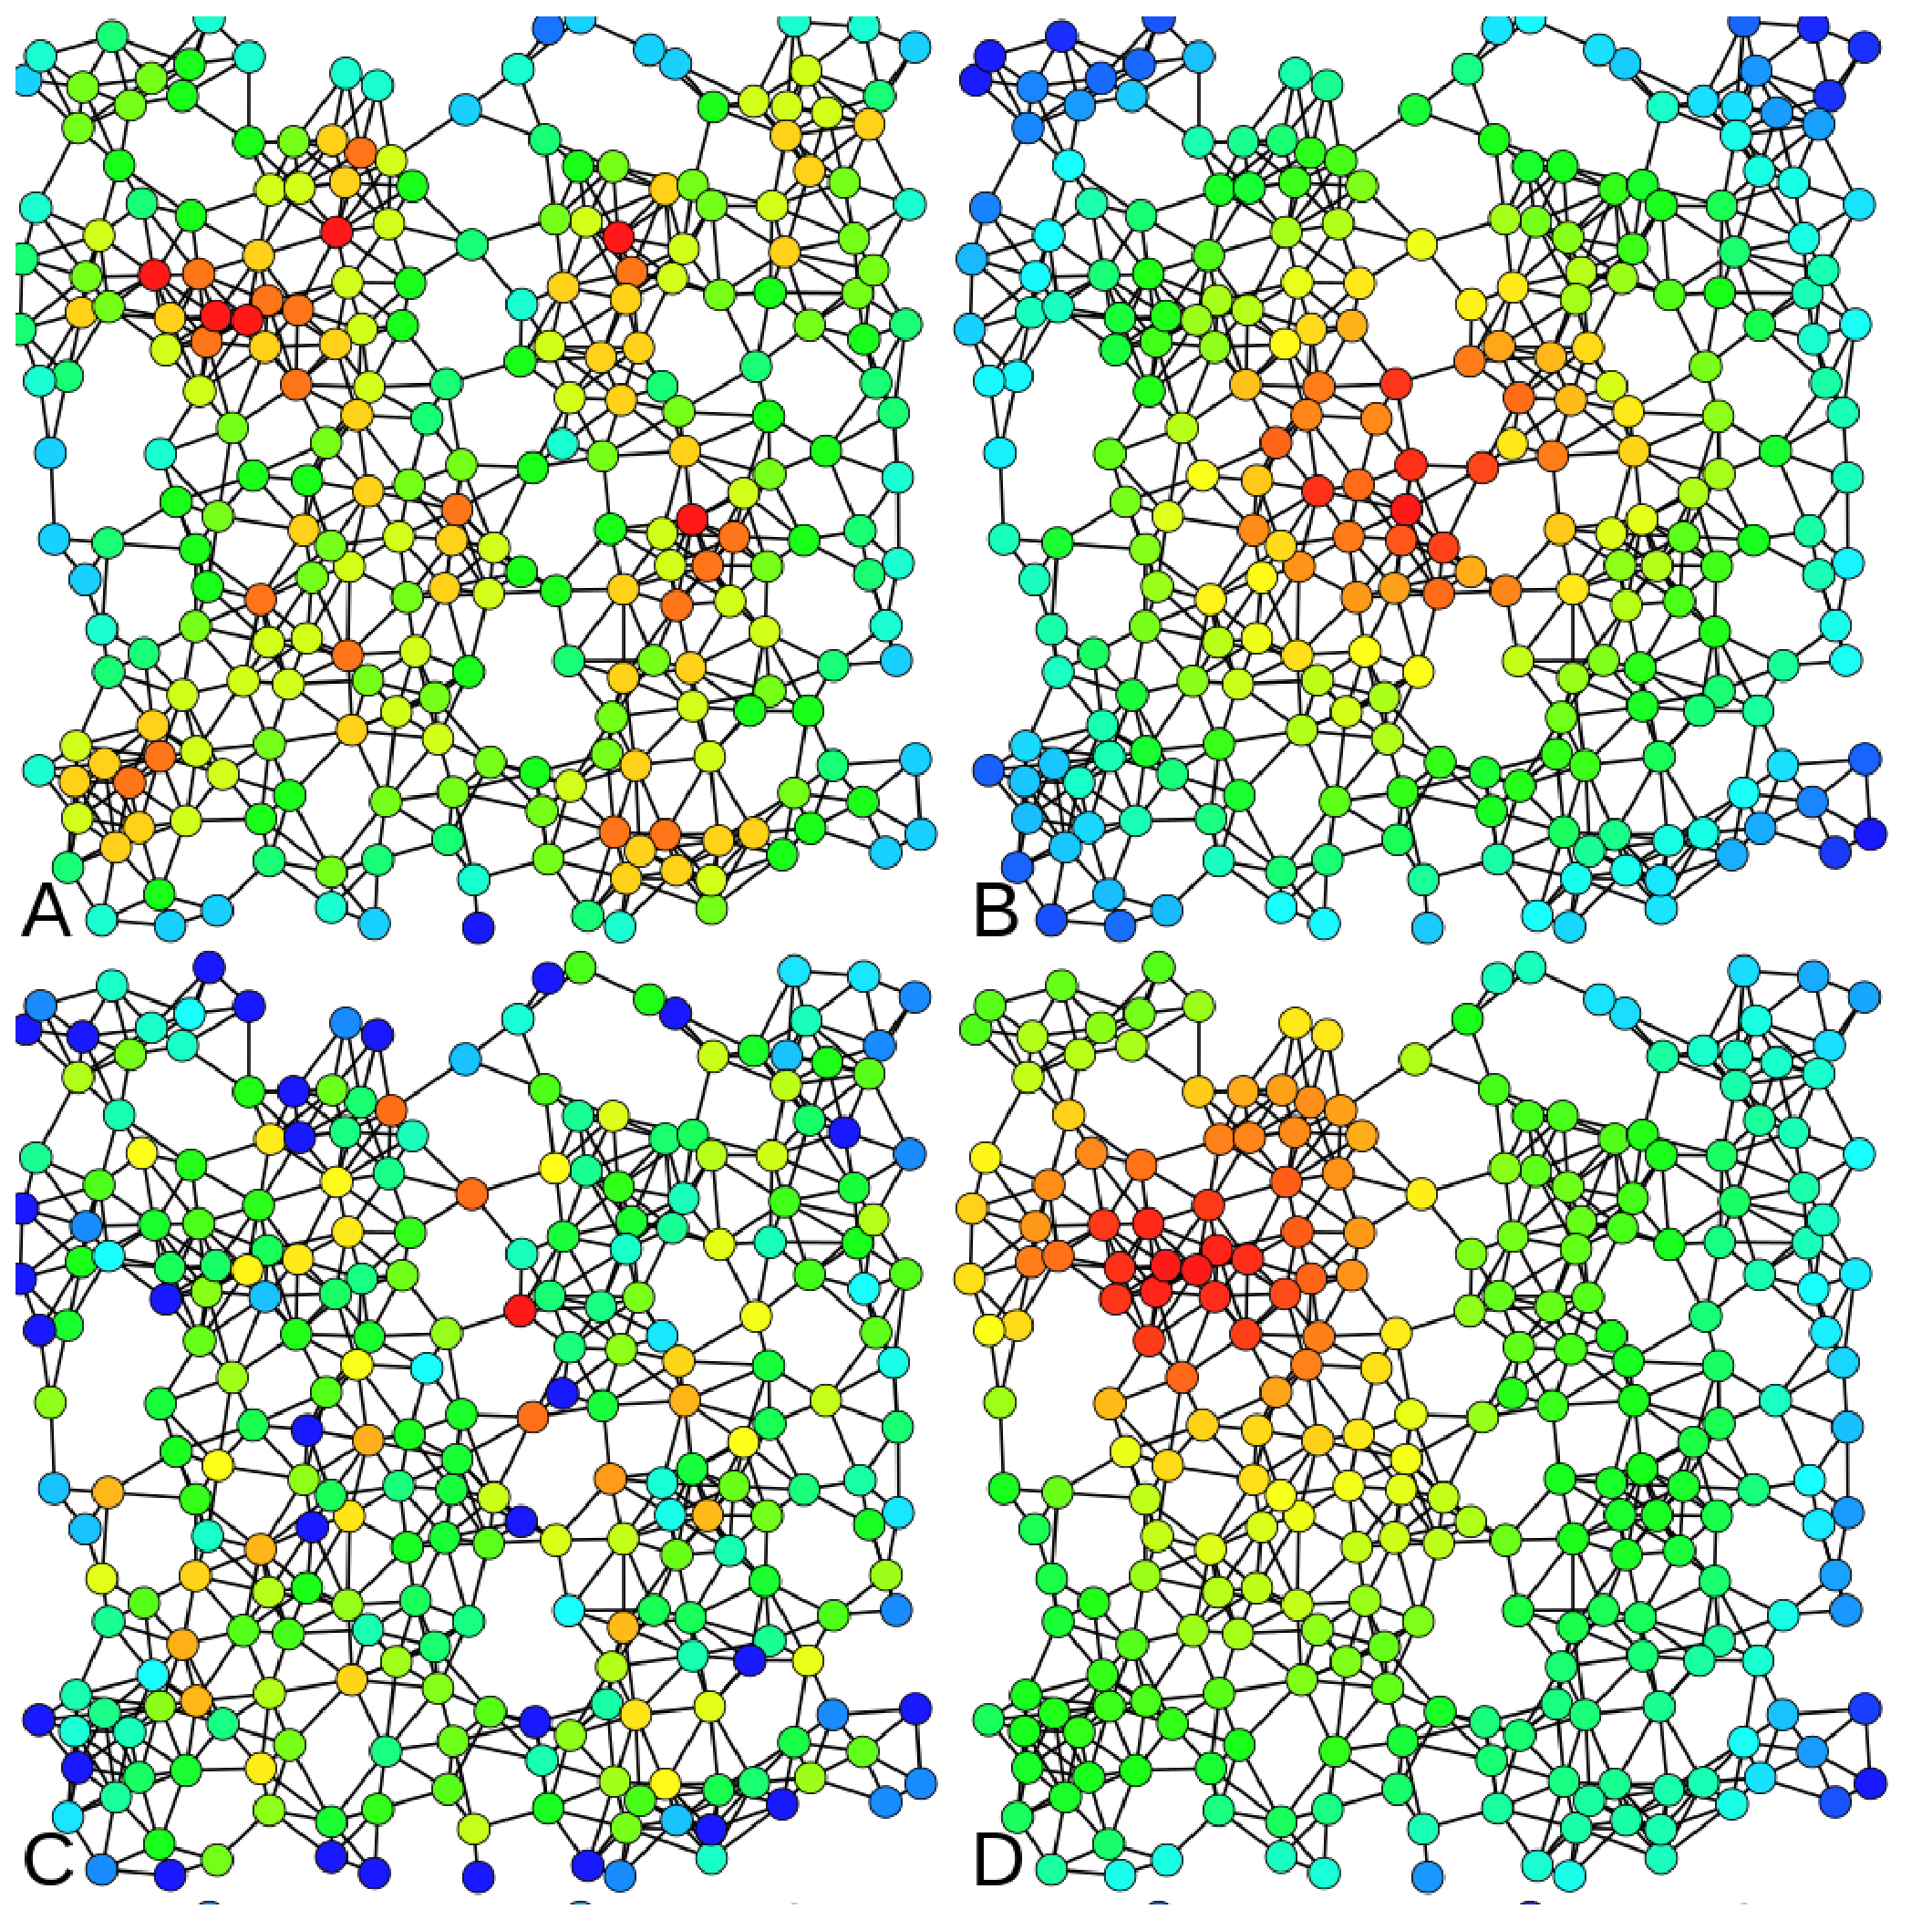
\epsfig{file=centrality.eps, width=0.7\columnwidth}
\caption[Heat-map color-coded examples Degree, Closeness, Betweenness, Eigenvector centralities]{Heat-map color-coded examples are shown above. Nodes with higher centrality metric are colored with warmer color: red is the warmest color here. The same network is analyzed four times with the following centrality measures:  A) Degree centrality, B) Closeness centrality, C) Betweenness centrality and D) Eigenvector centrality \cite{Rocchini}}
\label{figureCentrality}
\end{figure}

There are many ways of looking at an individual's importance/prestige/status within a network. One is called \textit{closeness centrality}. The \textit{farness} of a node is defined as the sum of its distances to all other nodes. The \textit{closeness} of a node is defined as the inverse of the farness. More informally, the more central a node is the lower its total distance to all other nodes. \textit{Closeness centrality} can be used as a measure of how fast information will spread through the network \cite{Chakrabarti}. Secondly, if we are looking for people who can serve as bridges between two distinct communities, we could measure the node's \textit{betweenness centrality}. Betweenness centralities for mediators who act as intermediate entities between other nodes are higher \cite{Chakrabarti}.  Third, if cross-community collaboration is the focus, we can measure \textit{edge betweenness centrality}.  Edges connecting nodes from different communities have higher edge centrality values. In the community collaboration graph, edge betweenness or stress of an edge is the number of these shortest paths that the edge belongs to, considering all shortest paths between all pairs of nodes in the graph. Fourth, one can claim that certain people in the community are more important than others, and whoever is close to them, is relatively more important than others. In graph terms, this is measured by \textit{eigenvector centrality}, which is based on the assumption that connections to high-profile nodes contribute more to the importance of a node. Google's PageRank link-analysis algorithm \cite{Page} is a variant of the eigenvector centrality measure. In short, centrality measures have been used in several studies to identify key player in a community.

In addition to the centrality measures, we planned to look into the \textit{resilience} of the community as well. By resilience, we mean how well the network holds its structure and form when some parts of it are deleted, added, or changed. For a graph, the resilience of a graph is a measure of its robustness to node or edge failures. This could occur for instance when an influential member of the community leaves. Many real-world graphs are resilient to random failures but vulnerable to targeted attacks. Resilience can be related to the \textit{graph diameter}: a graph whose diameter does not increase much on node or edge removal has higher resilience \cite{Chakrabarti}.

\subsection{Visualization}
Several visualization techniques and tools are used in the field of social network analysis, for instance, Gephi \cite{Bastian}, which is a FOSS tool for exploring and manipulating networks. It is capable of handling large networks with more than 20,000 nodes and features several SNA algorithms. We used it for dynamic network visualization.
We visualized the dynamic network changes using Gephi \cite{Bastian}. The videos\footnote{\label{footnote1}Video visualizations available at \href{http://eecs.oregonstate.edu/~azarbaam/OSS2014/}{http://eecs.oregonstate.edu/\textasciitilde azarbaam/OSS2014/}} show how the community graph is structured, using a continuous force-directed linear-linear model, in which the nodes are positioned near or far from one another proportional to the graph distance between them. This results in a graph shape between Fr\"{u}chterman \& Rheingold's \cite{Fruchterman} layout and Noack's LinLog \cite{Noack}.


\subsection{Initial study results and discussion}
\label{results}

\begin{figure}[!Ht]
\centering
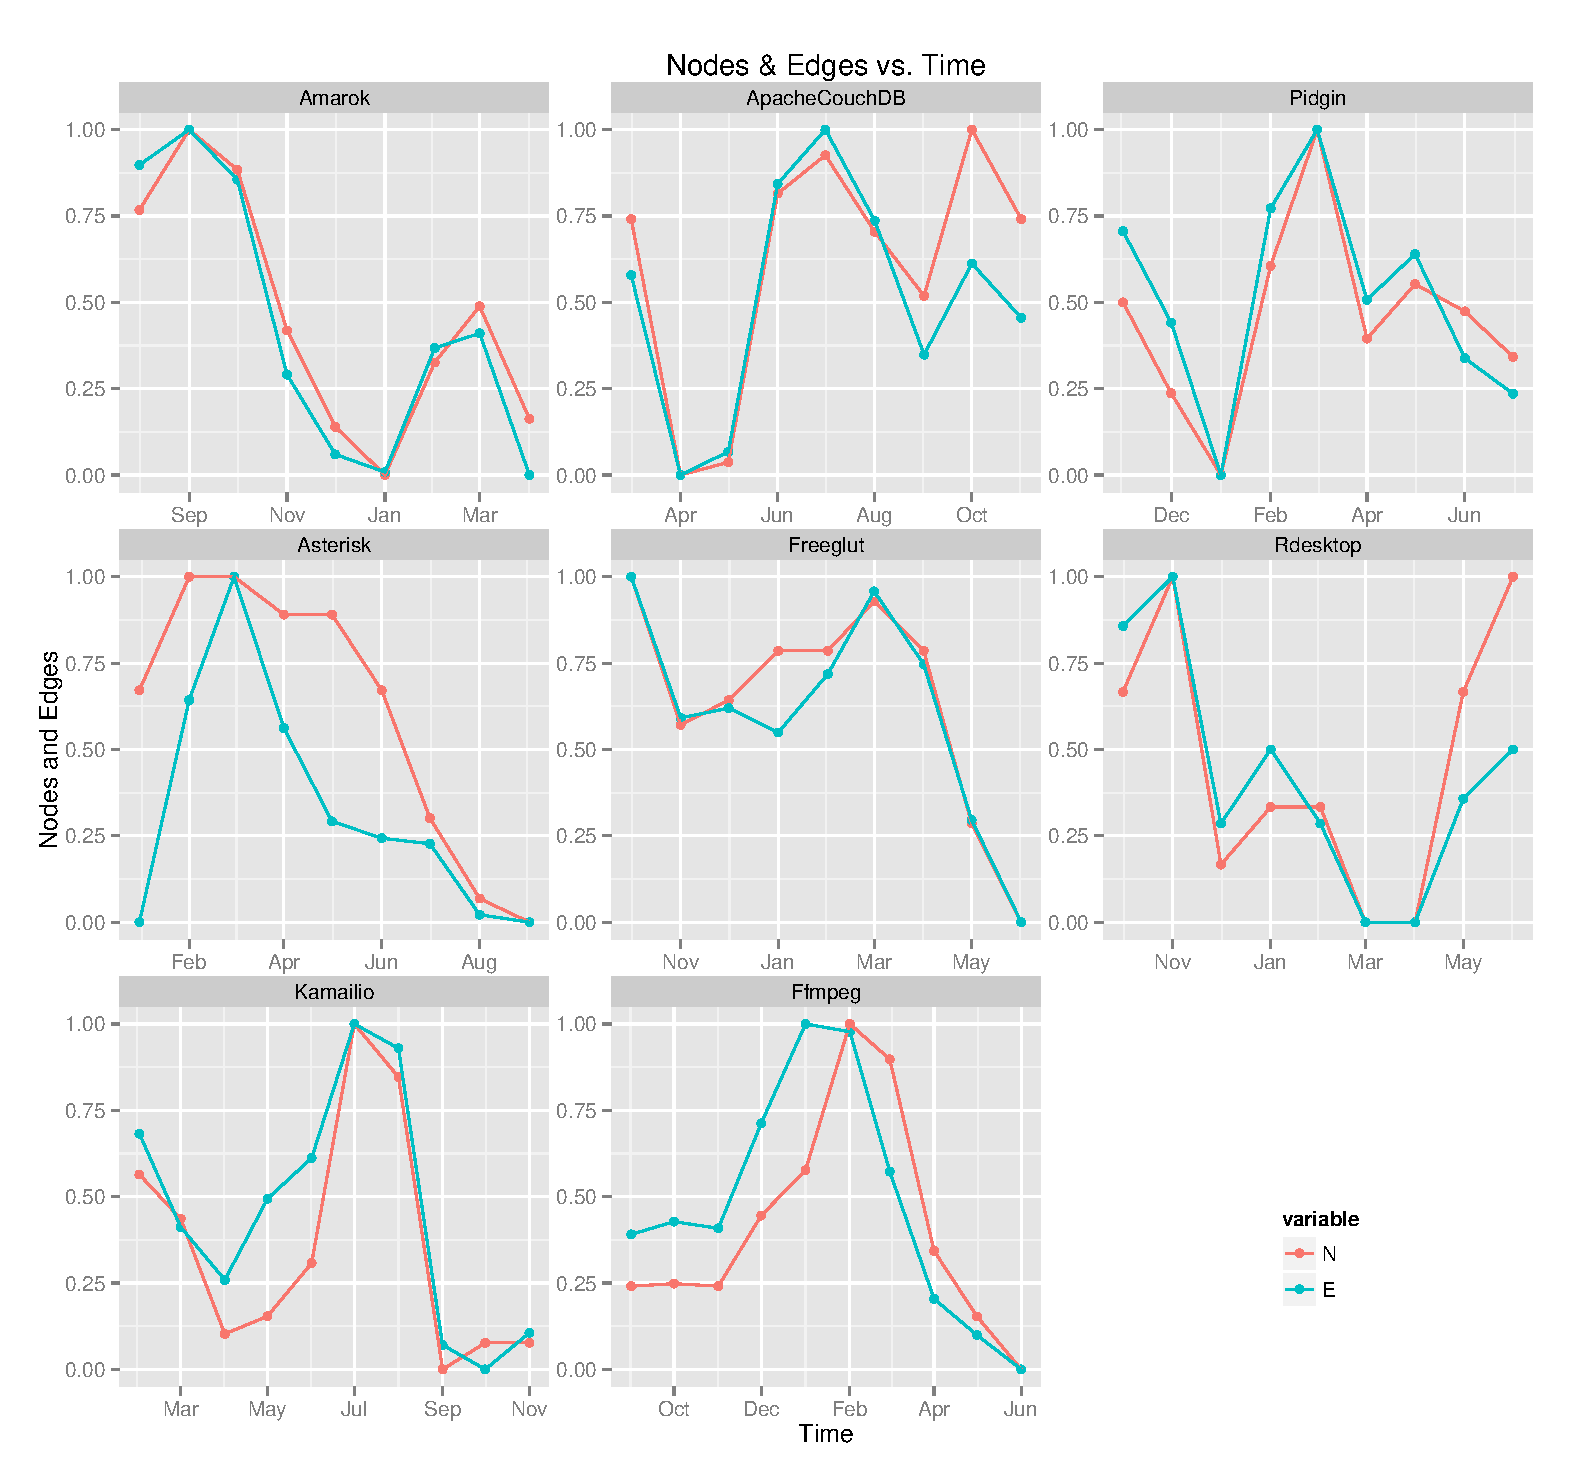
\epsfig{file=NodesEdgesTime.eps, width=\columnwidth}
\caption[The number of nodes and edges over time, as network-specific measurements]{Nodes and Edges over Time. The number of nodes and number of edges are normalized to the range [0,1] to make comparison across projects meaningful, by emphasizing change in ratio, rather than the varying counts. Hence, the measurements were normalized for drawing this graph. The three projects in the first row belong to the \textit{``technical differences''} forking reason category, the three projects in the second row belong to the \textit{``more community-driven development''} forking reason category, and the two projects in the third row belong to the \textit{``personal differences''} forking reason category.}
\label{figureNodesEdgesTimeR}
\end{figure}

\begin{figure}[!Ht]
\centering
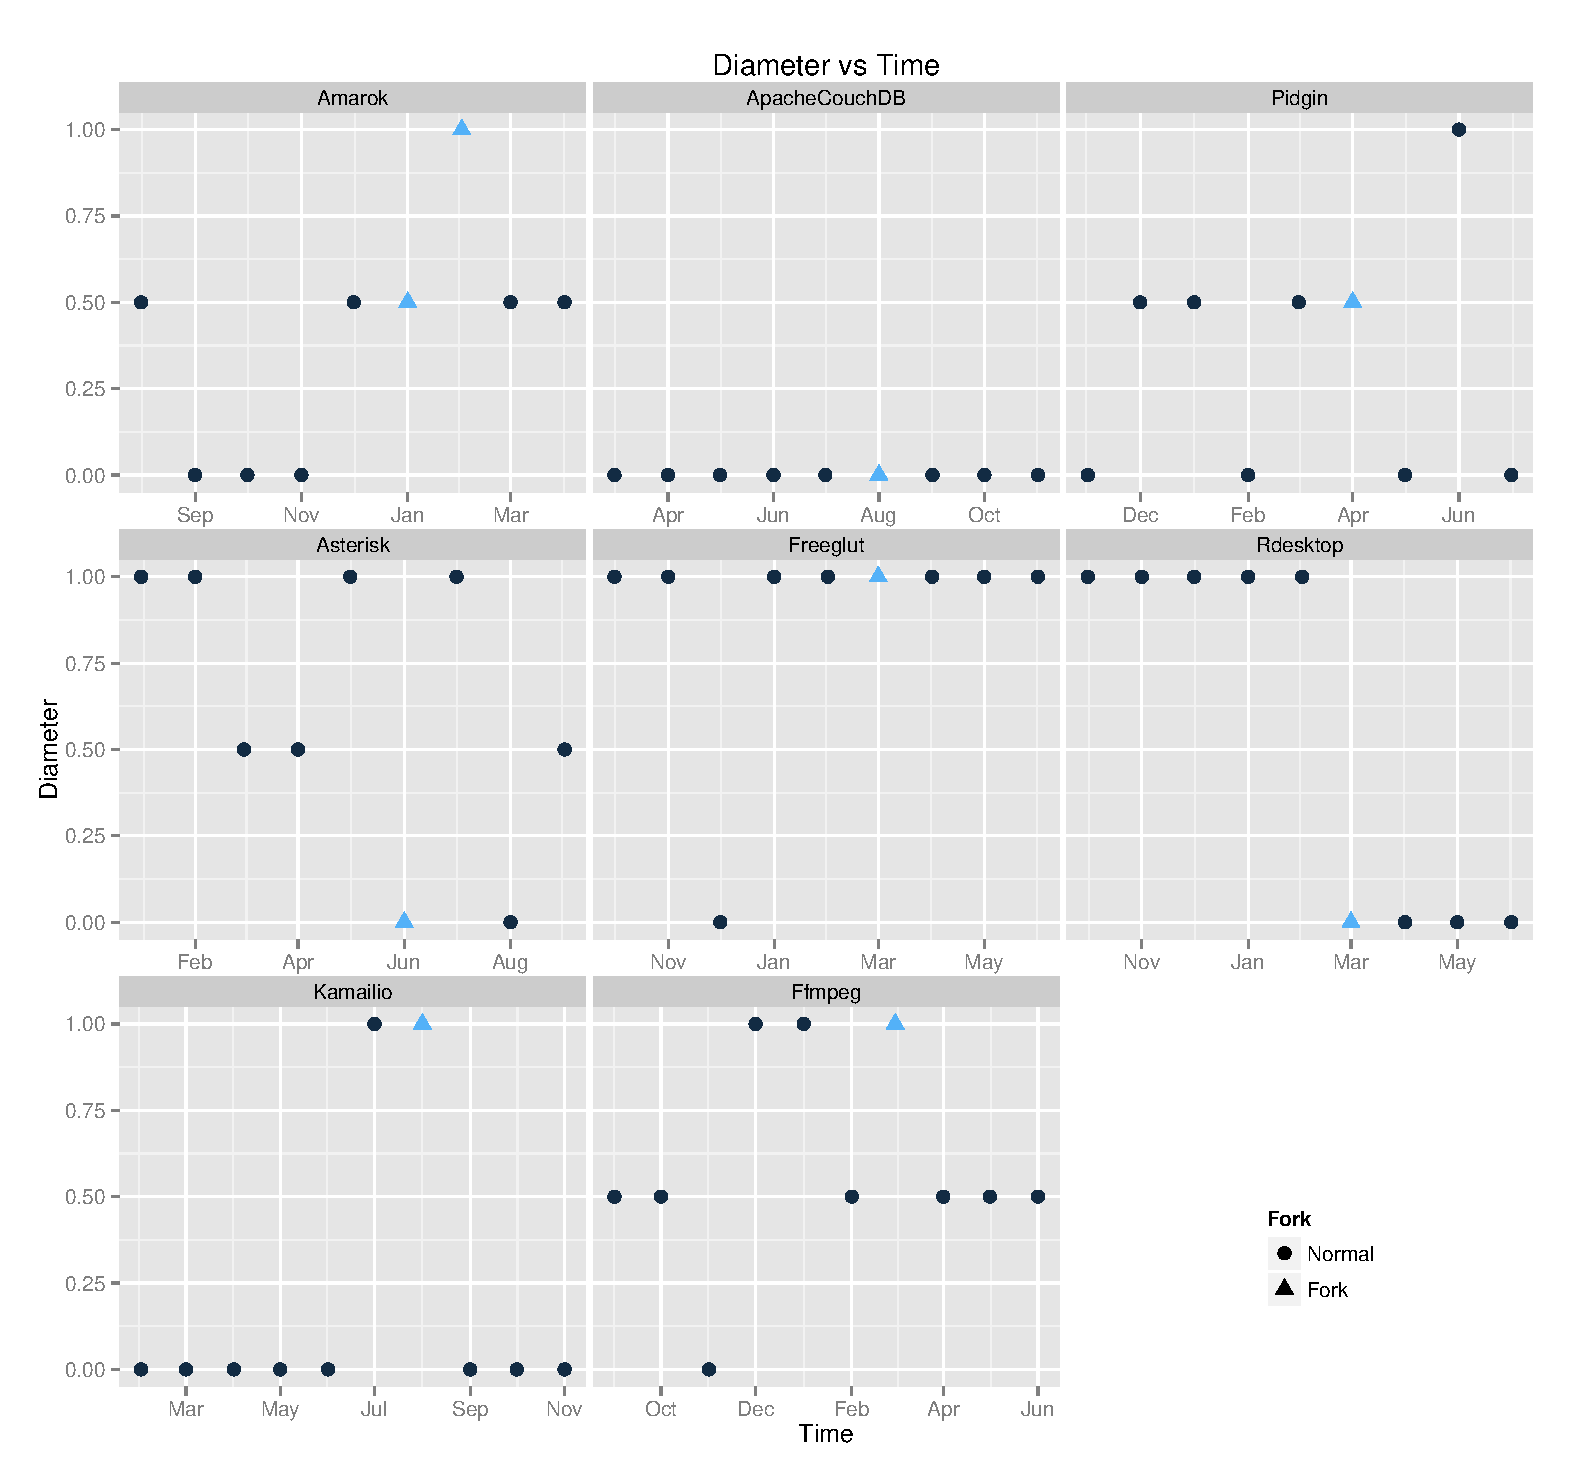
\epsfig{file=DiameterTime.eps, width=\columnwidth}
\caption[The network diameter change over time, as network-specific measurements]{Diameter changes over Time. Note that the diameter measurements were normalized to the range [0,1]. The three projects in the first row belong to the \textit{``technical differences''} forking reason category, the three projects in the second row belong to the \textit{``more community-driven development''} forking reason category, and the two projects in the third row belong to the \textit{``personal differences''} forking reason category.}
\label{figureDiameterTimeR}
\end{figure}

\subsubsection{Kamailio Project}
Figure \ref{figureKamailioGraph} shows four key frames from the Kamailio project's social graph around the time of their fork (the events described here are easier to fully grasp by watching the video. A node's size in a proportional to the number of interactions the node (contributor) has had within the study period and the position and edges of the nodes change if they had interactions within the time window shown, with six day steps per frame. The 1 minute and 37 seconds video shows the life of the Kamailio project between October 2007, and March 2009. Nodes are colored based on the modularity of the network. The community starts with the GeneralList as the the biggest node, and four larger core contributors and three lesser size core contributors. The big red-colored node's transitions are hard to miss, as this major contributor departs from the core to the periphery of the network (Video minute 1:02) and then leaves the community (Video minute 1:24) capturing either a conflict or retirement. This corresponds to the personal difference category of forking reasons.

\begin{figure*}[!htb]
\centering
\def\tabularxcolumn#1{m{#1}} 
\begin{tabularx}{\linewidth}{@{}cXX@{}}
\begin{tabular}{cccc} 
\subfloat[]{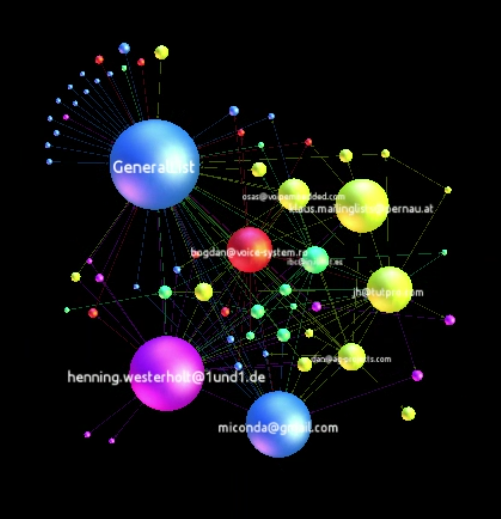
\includegraphics[width=0.25\textwidth, height=0.25\textwidth]{2}} 
&
\subfloat[]{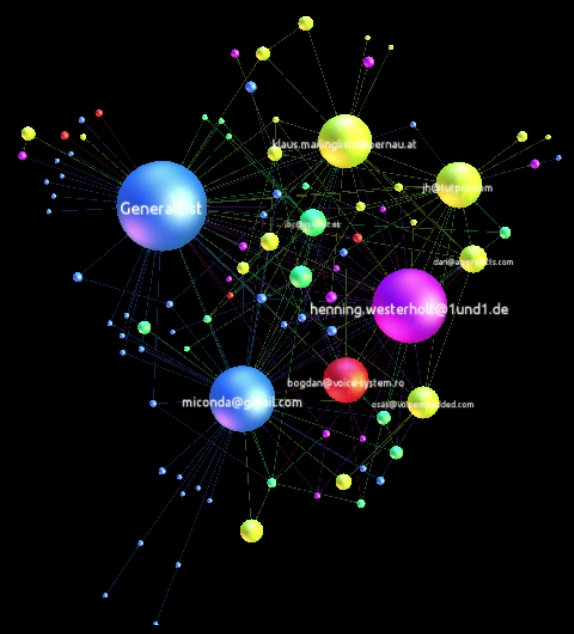
\includegraphics[width=0.25\textwidth, height=0.25\textwidth]{3}}
&
\subfloat[]{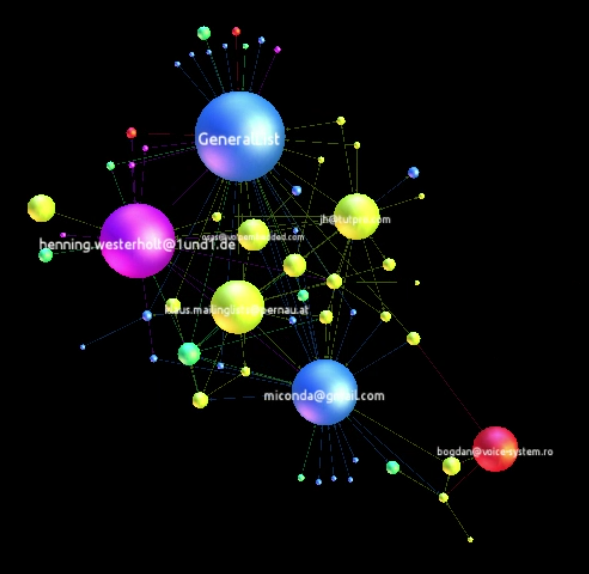
\includegraphics[width=0.25\textwidth, height=0.25\textwidth]{5}} 
& 
\subfloat[]{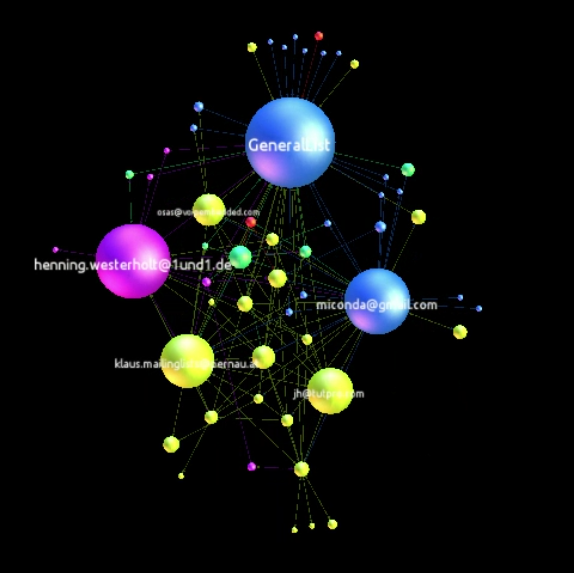
\includegraphics[width=0.25\textwidth, height=0.25\textwidth]{7}}
\end{tabular} 
\end{tabularx} 
\caption[Snapshots from video visualization of Kamailio project's graph]{Snapshots from video visualization of Kamailio's graph (Oct. 2007 - Mar. 2009) in which a core contributor (colored red) moves to the periphery and eventually departs the community.} 
\label{figureKamailioGraph} 
\end{figure*} 


\begin{figure*}[!htb]
\centering
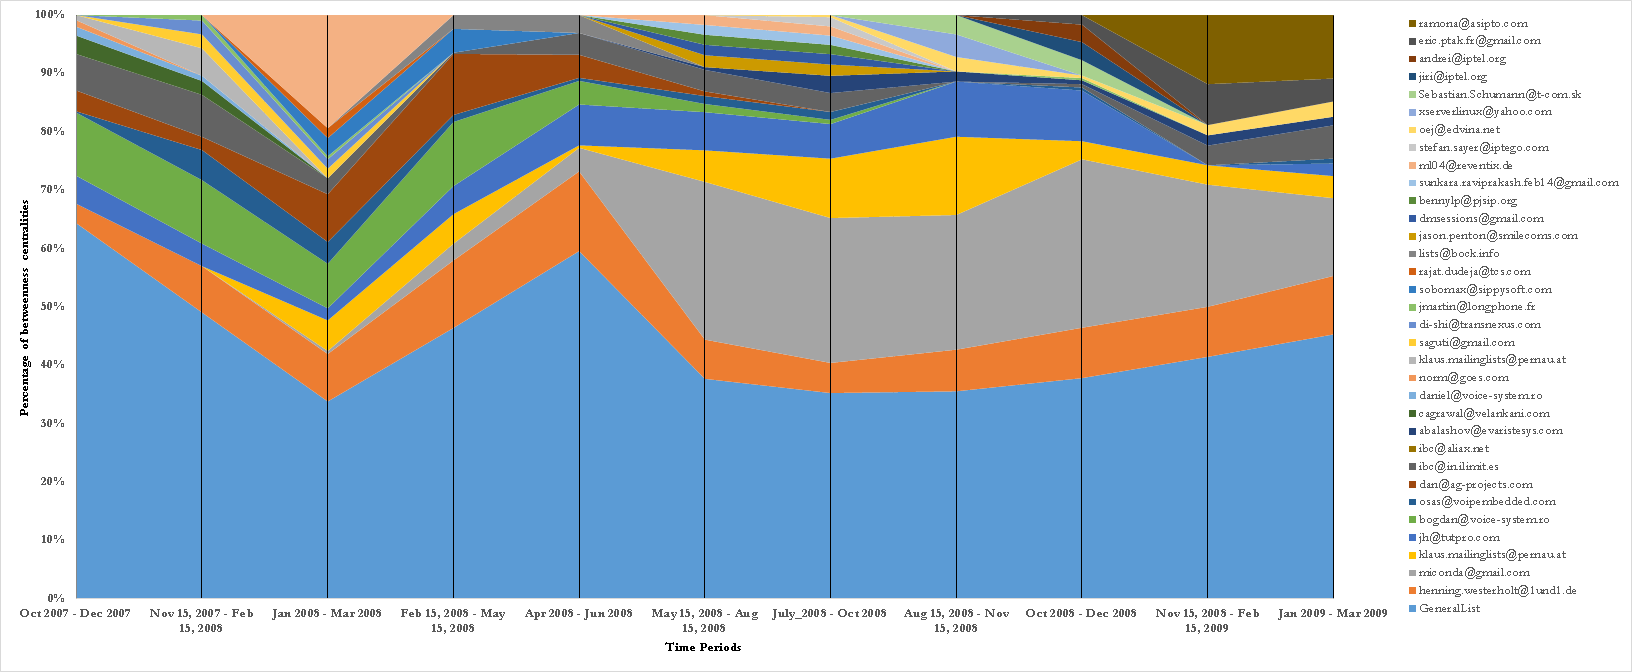
\epsfig{file=Kamailio_chart.eps, width=\textwidth}
\justifying
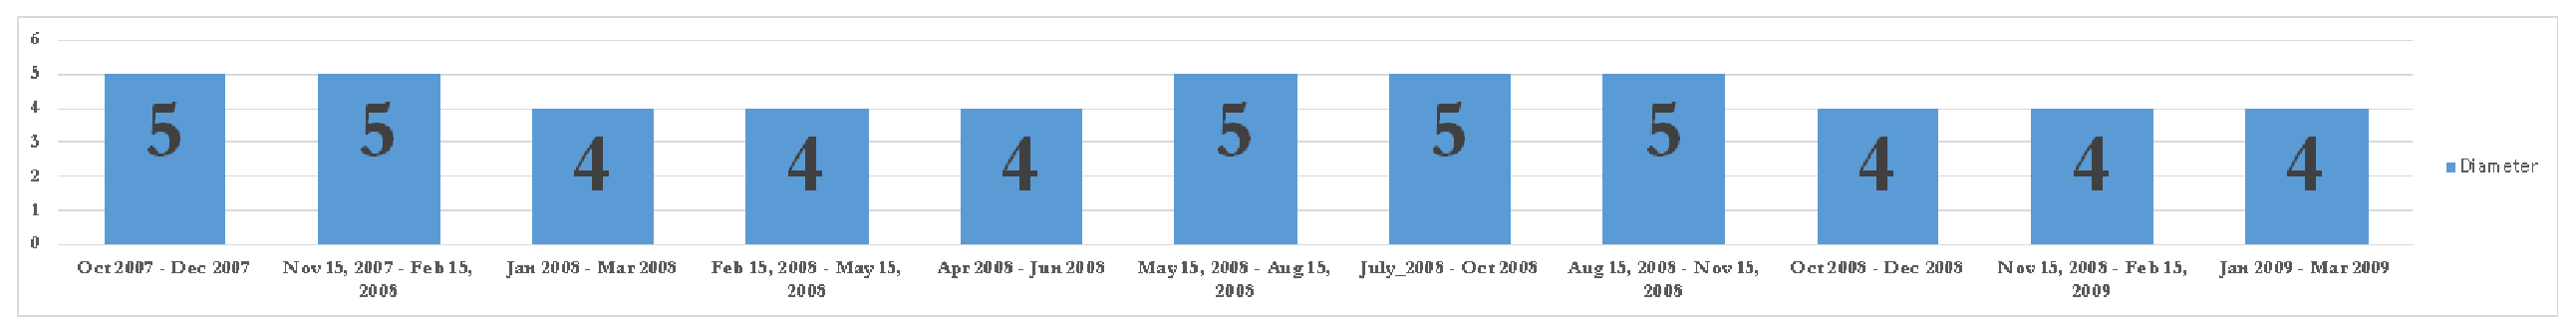
\epsfig{file=Kamailio_diameter.eps, width=\textwidth}
\caption[Kamailio top contributors' betweenness centralities and network diameter over time]{Kamailio top contributors' betweenness centralities and network diameter over time (Oct. 2007 to Mar. 2009) in 3-month time windows with 1.5-month overlaps}
\label{figureKamailioStackedAreaChart}
\end{figure*}

Figure \ref{figureKamailioStackedAreaChart} shows the betweenness centrality of the major contributors of Kamailio project over the same time period. The horizontal axis marks the dates, (each mark represents a 3-month time window with 1.5 months overlap). The vertical axis shows the percentage of the top betweenness centralities for each node. The saliency of the GeneralList -- colored as light blue -- is apparent because of its continuous and dominant presence in the stacked area chart. The chart legend lists the contributors based on the color and in the same order of appearance on the chart starting from the bottom. Around the "Aug. 15, 2008 - Nov. 15, 2008" tick mark on the horizontal axis, several contributors' betweenness centralities shrink to almost zero and disappear. This suggests the date of fork with a month accuracy. The network diameter of the Kamailio project over the same time period is also shown in Figure \ref{figureKamailioStackedAreaChart}. An increase in the network diameter during this period is noticeable; this coincides with findings of Hannemann and Klamma \cite{Hannemann}.

This technique can be used to identify the people involved in conflict and the date the fork happened with a months accuracy, even if the rival project does not emerge immediately.

\subsubsection{Amarok Project}
\begin{figure*}
\centering
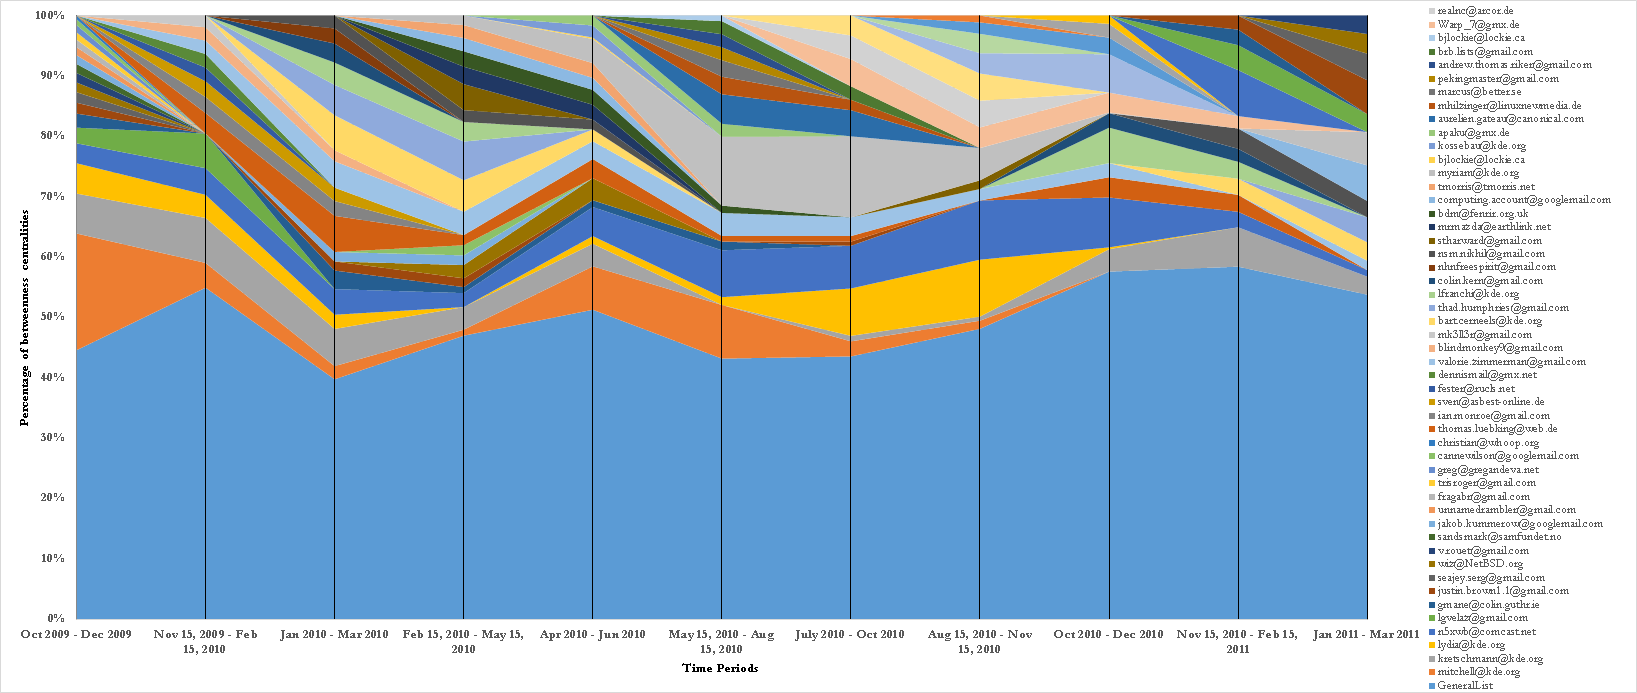
\epsfig{file=Amarok_chart.eps, width=\textwidth}
\justifying
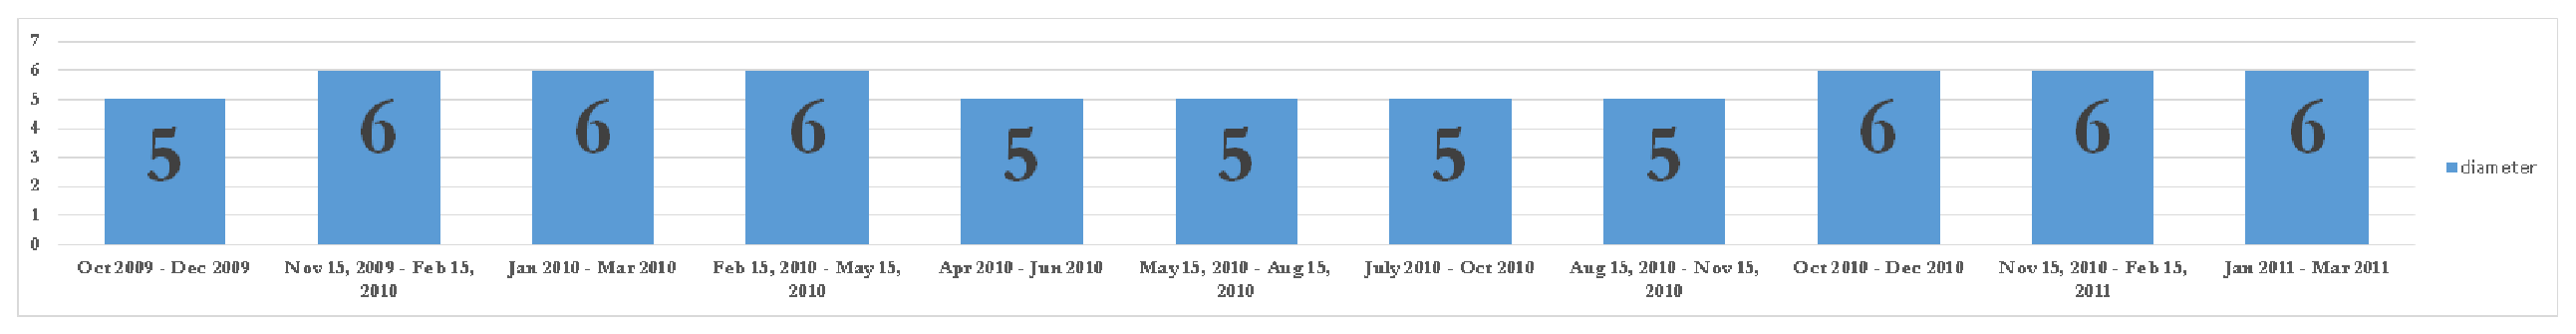
\epsfig{file=Amarok_diameter.eps, width=0.925\textwidth}
\caption[Amarok project's top contributors' betweenness centralities and network diameter over time]{Amarok project's top contributors' betweenness centralities and network diameter over time between Oct. 2009 to Mar. 2011 in 3-months time windows with 1.5 months overlaps}
\label{figureAmarokStachedAreaChart}
\end{figure*}

The video for the Amarok project fork is available online\footnote{Video visualizations available at \href{http://eecs.oregonstate.edu/~azarbaam/OSS2014/}{http://eecs.oregonstate.edu/\textasciitilde azarbaam/OSS2014/}}, and the results from our quantitative analysis of the betweenness centralities and the network diameters are shown in Figure \ref{figureAmarokStachedAreaChart}. The results show that the network diameter has not increased over the period of the fork, which shows a resilient network. The video shows the dynamic changes in the network structure, again typical of a healthy network, rather than of simmering conflict. These indicators suggest that the Amarok fork in 2010 belongs to the ``addition of technical functionality'' rationale for forking, as there are no visible social conflict.

\subsubsection{Asterisk Project}
\begin{figure*}
\centering
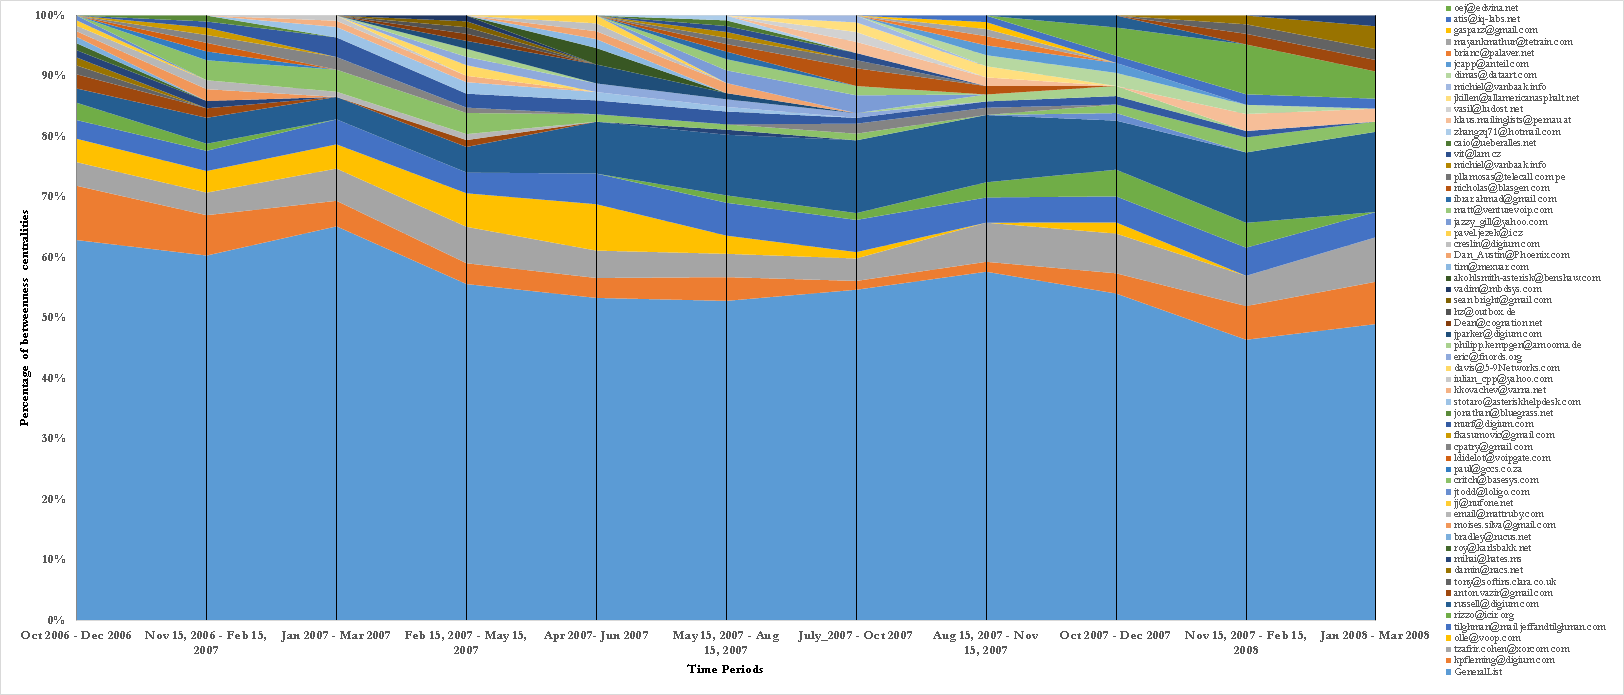
\epsfig{file=Asterisk_chart.eps, width=\textwidth}
\justifying
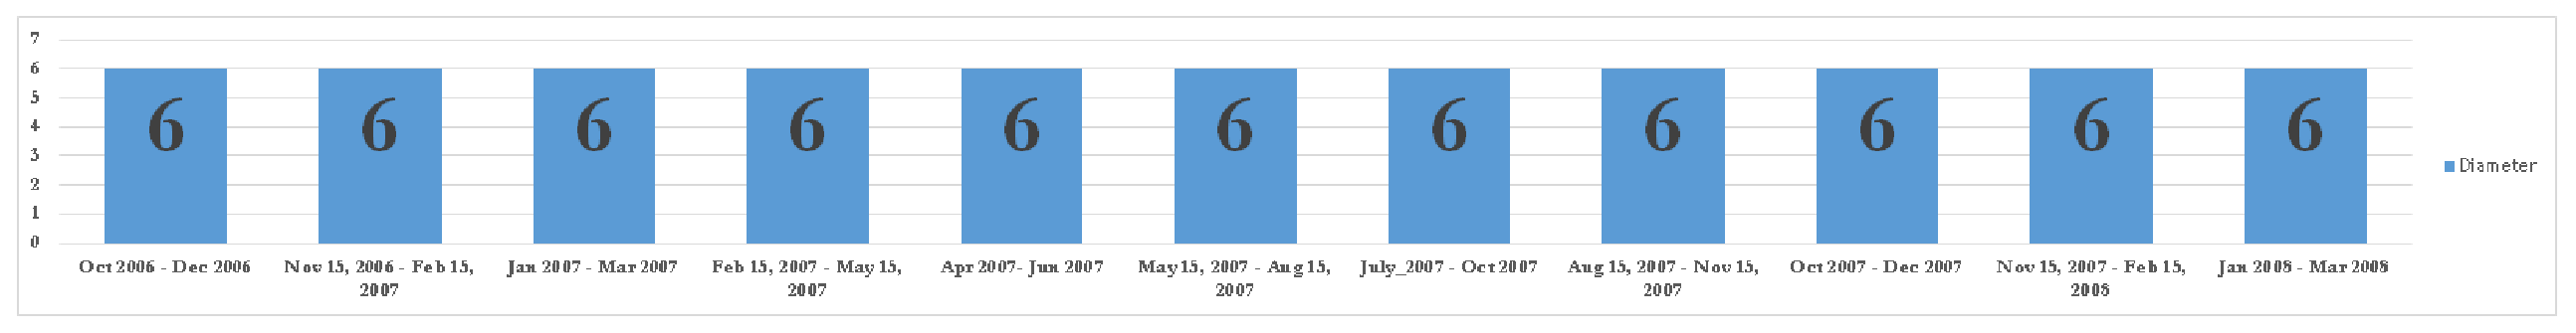
\epsfig{file=Asterisk_diameter.eps, width=0.94\textwidth}
\caption[Asterisk project's top contributors' betweenness centralities and network diameter over time]{Asterisk project's top contributors' betweenness centralities and network diameter over time between Oct. 2009 to Mar. 2011 in 3-months time windows with 1.5 months overlaps}
\label{figureAsteriskStackedAreaChart}
\end{figure*}

The video for the Asterisk project is also available online\footnote{Video visualizations available at \href{http://eecs.oregonstate.edu/~azarbaam/OSS2014/}{http://eecs.oregonstate.edu/\textasciitilde azarbaam/OSS2014/}}, and the results from our quantitative analysis of the betweenness centralities and the network diameters are shown in Figure \ref{figureAsteriskStackedAreaChart}. The results show that the network diameter remained steady at 6 throughout the period. The Asterisk community was by far the most crowded project, with 932 nodes and 4282 edges. The stacked area chart shows the distribution of centralities, where we see an 80\%-20\% distribution (i.e., 80\% or more of the activity is attributed to six major players, with the rest of the community accounting for only 20\%). This is evident in the video representation as well, as the top-level structure of the network holds throughout the time period. The results from the visual and quantitative analysis links the Asterisk fork to the more community-driven category of forking reasons.

\subsubsection{Initial study conclusion}
We studied the collaboration networks of three FOSS projects using a combination of temporal visualization and quantitative analysis. We based our study on two papers by Robles and Gonzalez-Barahona \cite{Robles} and Hannemann and Klamma \cite{Hannemann}, and identified three projects that had forked in the recent past. We mined the collaboration data, formed dynamic collaboration graphs, and measured social network metrics over an 18-month period time window.

We also visualized the dynamic graphs (available online) and as stacked area charts over time. The visualizations and the quantitative results showed the differences among the projects in the three forking reasons of personal differences among the developer teams, technical differences (addition of new functionality) and more community-driven development. The novelty of the approach was in applying the network-specific \textit{temporal} analysis rather than static analysis, and in the temporal visualization of community structure. We showed that this approach shed light on the structure of these projects and reveal information that cannot be seen otherwise.\\

More importantly, the initial study showed the limitations of a \textit{network-specific} approach, and hence, we adopted a \textit{population-processes} approach for our main study as explained in section \ref{relatedwork}.

\end{appendices}

\pagebreak




%%%%%%%%%%%%%%%%%%%%%%%% referenc.tex %%%%%%%%%%%%%%%%%%%%%%%%%%%%%%
% sample references
% "computer science"
%
% Use this file as a template for your own input.
%
%%%%%%%%%%%%%%%%%%%%%%%% Springer-Verlag %%%%%%%%%%%%%%%%%%%%%%%%%%
%
% BibTeX users please use
% \bibliographystyle{}
% \bibliography{}
%
% Non-BibTeX users please use
\begin{thebibliography}{99.}
%
% and use \bibitem to create references.
%
% Use the following syntax and markup for your references
%
%% Monographs
%\bibitem{monograph} Kajan E (2002)
%Information technology encyclopedia and acronyms. Springer, Berlin
%Heidelberg New York
%
%% Contributed Works
%\bibitem{contribution} Broy M (2002) Software engineering -- From
%auxiliary to key technologies. In: Broy M, Denert E (eds)
%Software Pioneers. Springer, Berlin Heidelberg New York
%
%% Journal
%\bibitem{journal} Che M, Grellmann W, Seidler S (1997)
%Appl Polym Sci 64:1079--1090
%
%\bibitem{journal} Chde M, Grellmann W, Seidler S (1997)
%Appl Polym Sci 64:1079--1090
%
%%% Theses
%%\bibitem{thesis} Ross DW (1977) Lysosomes and storage diseases. MA
%%Thesis, Columbia University, New York
%
\bibitem{Asur} Asur, S., S. Parthasarathy, and D. Ucar, (2009), ``\textit{An event-based framework for characterizing the evolutionary behavior of interaction graphs,}'' ACM Trans.  Knowledge Discovery Data. 3, 4, Article 16, (November 2009), 36 pages. 2009.

\bibitem{AzarbakhtOSS2014} Azarbakht, A. and C. Jensen, ``\textit{Drawing the Big Picture: Temporal Visualization of Dynamic Collaboration Graphs of OSS Software Forks,}'' Proc. 10th Int'l. Conf. Open Source Systems, 2014.

\bibitem{AzarbakhtINSNA2014} Azarbakht, A. and C. Jensen, ``\textit{Temporal Visualization of Dynamic Collaboration Graphs of OSS Software Forks,}'' Proc. Int'l. Network for Social Network Analysis (INSNA) Sunbelt XXXIV Conf., 2014.

\bibitem{AzarbakhtOpenSym2013} Azarbakht, A., ``\textit{Drawing the Big Picture: Analyzing FLOSS Collaboration with Temporal Social Network Analysis,}'' Proc. 9th Int'l. Symp. Open Collaboration, ACM, 2013.

\bibitem{AzarbakhtOSS2013} Azarbakht, A. and C. Jensen, ``\textit{Analyzing FOSS Collaboration \& Social Dynamics with Temporal Social Networks,}'' Proc. 9th Int'l. Conf. Open Source Systems Doct. Cons., 2013.

\bibitem{AzarbakhtVLHCC2014} Azarbakht, A., ``\textit{Temporal Visualization of Collaborative Software Development in FOSS Forks,}'' Proc. IEEE Symp. Visual Languages and Human-Centric Computing, 2014.

\bibitem{Baishakhi} Baishakhi R., C. Wiley, and M. Kim, ``\textit{REPERTOIRE: a cross-system porting analysis tool for forked software projects,}'' Proc. ACM SIGSOFT 20th Int'l. Symp. Foundations of Software Engineering, ACM, 2012.

\bibitem{Bastian} Bastian, M., S. Heymann, and M. Jacomy, ``\textit{Gephi: an open source software for exploring and manipulating networks,}'' Int'l AAAI Conf. on Weblogs and Social Media, 2009.

\bibitem{Bezrukova} Bezrukova, K,, C. S. Spell, J. L. Perry, ``\textit{Violent Splits Or Healthy Divides? Coping With Injustice Through Faultlines,}'' Personnel Psychology, Vol 63, Issue 3. 2010. 

\bibitem{Bird} Bird, C., D. Pattison, R. D'Souza, V. Filkov, and P. Devanbu, ``\textit{Latent social structure in open source projects,}'' Proc. 16th ACM SIGSOFT Int'l. Symposium on Foundations of software engineering, ACM, 2008.  

\bibitem{Brandes} Brandes, U. ``\textit{A Faster Algorithm for Betweenness Centrality}'', Journal of Mathematical Sociology 25(2):163-177, 2001.

\bibitem{Chakrabarti} Chakrabarti,  D., and C. Faloutsos. ``\textit{Graph mining: Laws, generators, and algorithms,}'' ACM Computing Surveys, 38, 1, Article 2, 2006.

\bibitem{Coleman1964} Coleman, J.S. ``\textit{Introduction to Mathematical Sociology,}'' New York etc.: The Free Press of Glencoe. 1964.

\bibitem{CrowstonFLOSSWhatWeKnow} 
Crowston, K., K. Wei, J. Howison, and A. Wiggins. ``\textit{Free/Libre open-source software development: What we know and what we do not know,}'' ACM Computing Surveys, 44, 2, Article 7, 2012.

\bibitem{DavidsonVLHCC2014} Davidson, J, R. Naik, A. Mannan, A. Azarbakht, C. Jensen, ``\textit{On older adults in free/open source software: reflections of contributors and community leaders,}'' Proc. IEEE Symp. Visual Languages and Human-Centric Computing, 2014.

\bibitem{Ernst} Ernst, N., S. Easterbrook, and J. Mylopoulos, ``\textit{Code forking in open-source software: a requirements perspective,}'' arXiv preprint arXiv:1004.2889, 2010.

\bibitem{Ford} Ford, L. R. and D. R. Folkerson, ``\textit{A simple algorithm for finding maximal network flows and an application to the Hitchcock problem,}'' Canadian Journal of Mathematics, vol. 9, pp. 210-218, 1957. 

\bibitem{Forrest} Forrest, D., C. Jensen, N. Mohan, and J. Davidson, ``\textit{Exploring the Role of Outside Organizations in Free/ Open Source Software Projects,}'' Proc. 8th Int'l. Conf. Open Source Systems, 2012.

\bibitem{Fruchterman} Fruchterman, T. M. J. and E. M. Reingold, ``\textit{Graph drawing by force-directed placement,}'' Softw: Pract. Exper., vol. 21, no. 11, pp. 1129-1164, 1991.

\bibitem{Guzzi} Guzzi, A., A. Bacchelli, M. Lanza, M. Pinzger, and A. van Deursen. ``\textit{Communication in open source software development mailing lists,}'' Proc. 10th Conf. on Mining Software Repositories, IEEE Press, 2013.

\bibitem{Hannemann} Hannemann, A and , R. Klamma ``\textit{Community Dynamics in Open Source Software Projects: Aging and Social Reshaping,}'' Proc. Int. Conf. on Open Source Systems, 2013. 

\bibitem{Heider} Heider, F. The Psychology of Interpersonal Relations. John Wiley \& Sons. 1958.

\bibitem{HowisonPerilsSourceForge} Howison, J. and K. Crowston. ``\textit{The perils and pitfalls of mining SourceForge,}'' Proc. Int'l. Workshop on Mining Software Repositories, 2004.  

\bibitem{HowisonSocialDynamics} Howison, J., K. Inoue, and K. Crowston, ``\textit{Social dynamics of free and open source team communications,}'' Proc. Int'l. Conf. Open Source Systems, 2006.  

\bibitem{HowisonFlossMole} Howison, J., M. Conklin, and K. Crowston, ``\textit{FLOSSmole: A collaborative repository for FLOSS research data and analyses,}'' Int'l. Journal of Information Technology and Web Engineering, 1(3), 17-26. 2006.

\bibitem{Krivitsky} Krivitsky, P. N., and M. S. Handcock. ``\textit{A separable model for dynamic networks,}'' Journal of the Royal Statistical Society: Series B (Statistical Methodology) 76, no. 1: 29-46. 2014.

\bibitem{Kuechler} Kuechler, V., C. Gilbertson, and C. Jensen, ``\textit{Gender Differences in Early Free and Open Source Software Joining Process,}'' Open Source Systems: Long-Term Sustainability, 2012. 

\bibitem{Kunegis} Kunegis, J., S. Sizov, F. Schwagereit, and D. Fay, ``\textit{Diversity dynamics in online networks,}'' Proc. 23rd ACM Conf. on Hypertext and Social Media, 2012. 

\bibitem{LeskovecGraphsOverTime} Leskovec, J., Kleinberg, J., and Faloutsos, C.: ``\textit{Graphs over time: densification laws, shrinking diameters and possible explanations,}'' Proc. SIGKDD Int'l. Conf. Knowledge Discovery and data Mining, 2005. 

\bibitem{LeskovecStatisticalPropertiesOfCommunityStructure} Leskovec, J., K. J. Lang, A. Dasgupta, and M. W. Mahoney, ``\textit{Statistical properties of community structure in large social and information networks,}'' Proc. 17th Int'l. Conf. World Wide Web, ACM, 2008.  

\bibitem{Nakakoji} Nakakoji, K., Y. Yamamoto, Y. Nishinaka, K. Kishida, and Y. Ye. ``\textit{Evolution patterns of open-source software systems and communities,}'' Proc. Int'l. Workshop Principles of Software Evolution, ACM, 2002.

\bibitem{NymanToForkOrNotToFork} Mikkonen, T., L. Nyman, ``\textit{To Fork or Not to Fork: Fork Motivations in SourceForge Projects,}'' Int'l. J. Open Source Softw. Process. 3, 3. July, 2011.

\bibitem{Noack} Noack, A., ``\textit{Energy models for graph clustering,}'' J. Graph Algorithms Appl., vol. 11, no. 2, pp. 453-480, 2007.

\bibitem{Nowak} Nowak, M. A. ``\textit{Five rules for the evolution of cooperation,}'' Science 314, No. 5805: 1560-1563. 2006.

\bibitem{NymanCodeForking} Nyman, L. , ``\textit{Understanding code forking in open source software,}'' Proc. 7th Int'l. Conf. Open Source Systems Doct. Cons., 2011. 

\bibitem{NymanForkingSustainability} Nyman, L., T. Mikkonen, J. Lindman, and M. Foug\`{e}re, ``\textit{Forking: the invisible hand of sustainability in open source software,}'' Proc. SOS 2011: Towards Sustainable Open Source, 2011. 

\bibitem{NymanHackersForking} Nyman, L., ``\textit{Hackers on Forking,}'' Proc. Int'l. Symp. on Open Collaboration, 2014. 

\bibitem{Oh} Oh, W., Jeon, S., ``\textit{Membership Dynamics and Network Stability in the Open-Source Community: The Ising Perspective}'' Proc. 25th Int'l. Conf. Information Systems. 2004.

\bibitem{Page} Page, B, B. Sergey, R. Motwani and T. Winograd, ``\textit{The PageRank Citation Ranking: Bringing Order to the Web,}'' Technical Report, Stanford InfoLab, 1999.

\bibitem{Robins} Robins, G., P. Pattison, Y. Kalish, and D. Lusher. ``\textit{An introduction to exponential random graph (p*) models for social networks,}'' Social networks 29, no. 2: 173-191. 2007.

\bibitem{Robles} Robles, G. and J. M. Gonzalez-Barahona, ``\textit{A comprehensive study of software forks: Dates, reasons and outcomes,}'' Proc. 8th Int'l. Conf. Open Source Systems, 2012. 

\bibitem{Rocchini} Rocchini, C. (Nov. 27 2012), Wikimedia Commons, Available:\\ http://en.wikipedia.org/wiki/File:Centrality.svg, 2012.  

\bibitem{Singer} Singer, L., F. Figueira Filho, B. Cleary, C. Treude, M. Storey, and K. Schneider. ``\textit{Mutual assessment in the social programmer ecosystem: an empirical investigation of developer profile aggregators,}'' Proc. Conf. Computer supported cooperative work, ACM, 2013.

\bibitem{SnijdersMCMCMLE} Snijders, T. AB. ``\textit{Markov chain Monte Carlo estimation of exponential random graph models,}'' Journal of Social Structure 3, no. 2: 1-40. 2002.

\bibitem{Snijders2004} Snijders, Tom AB. ``\textit{Models for longitudinal network data,}'' Models and methods in social network analysis 1 (2005): 215-247. 

\bibitem{Snijders2010} Snijders, Tom AB., GG Van de Bunt, CEG Steglich, ``\textit{Introduction to stochastic actor-based models for network dynamics,}'' Social networks 32 (1), 44-60. 2010.

\bibitem{Sowe} Sowe, S., L. Stamelos, and L. Angelis, ``\textit{Identifying knowledge brokers that yield software engineering knowledge in OSS projects,}'' Information and Software Technology, vol. 48, pp. 1025-1033, Nov 2006. 

\bibitem{Spence} Spence, M. ``\textit{Job market signaling,}'' Quarterly Journal of Economics, 87: 355-374. 1973.

\bibitem{Steglich} Steglich, C., T. AB Snijders, and M. Pearson. ``\textit{Dynamic networks and behavior: Separating selection from influence,}'' Sociological methodology 40, no. 1: 329-393. 2010.

\bibitem{Storey} Storey, M., L. Singer, B. Cleary, F. Figueira Filho, and A. Zagalsky, ``\textit{The (R) Evolution of social media in software engineering,}'' Proc. Future of Software Engineering, ACM, 2014.

\bibitem{Syeed} Syeed, M. M., ``\textit{Socio-Technical Dependencies in Forked OSS Projects: Evidence from the BSD Family,}'' Journal of Software 9.11 (2014): 2895-2909. 2014.

\bibitem{JoseWebKit} Teixeira, J., and T. Lin, ``\textit{Collaboration in the open-source arena: the webkit case,}'' Proc. 52nd ACM conf. Computers and people research (SIGSIM-CPR '14). ACM, 2014.

\bibitem{Torres} Torres, M. R. M., S. L. Toral, M. Perales, and F. Barrero, ``\textit{Analysis of the Core Team Role in Open Source Communities,}'' Int. Conf. on Complex, Intelligent and Software Intensive Systems, IEEE, 2011. 

\bibitem{Zachary} Zachary, W., ``\textit{An information flow model for conflict and fission in small groups,}'' Journal of Anthropological Research, vol. 33, no. 4, pp. 452-473, 1977.

\end{thebibliography}

\bibliography{referenc}  

% sigproc.bib is the name of the Bibliography in this case
% You must have a proper ".bib" file
%  and remember to run:
% latex bibtex latex latex
% to resolve all references
%
% ACM needs 'a single self-contained file'!
%
%APPENDICES are optional
%\balancecolumns
%\appendix
%%Appendix A
%\section*{Appendix A: Table of all U.F. projects}


%%%%%%%%%%%%%%%%%%%%%%%%%%%%%%%%%%%%%%%%%%%%
%The rules about hierarchical headings discussed above for 
%the body of the article are different in the appendices.
%In the \textbf{appendix} environment, the command
%\textbf{section} is used to
%indicate the start of each Appendix, with alphabetic order
%designation (i.e. the first is A, the second B, etc.) and
%a title (if you include one).  So, if you need
%hierarchical structure
%\textit{within} an Appendix, start with \textbf{subsection} as the
%highest level. Here is an outline of the body of this
%document in Appendix-appropriate form:
%\subsection{Introduction}
%\subsection{The Body of the Paper}
%\subsubsection{Type Changes and  Special Characters}
%\subsubsection{Math Equations}
%\paragraph{Inline (In-text) Equations}
%\paragraph{Display Equations}
%\subsubsection{Citations}
%\subsubsection{Tables}
%\subsubsection{Figures}
%\subsubsection{Theorem-like Constructs}
%\subsubsection*{A Caveat for the \TeX\ Expert}
%\subsection{Conclusions}
%\subsection{Acknowledgments}
%\subsection{Additional Authors}
%This section is inserted by \LaTeX; you do not insert it.
%You just add the names and information in the
%\texttt{{\char'134}additionalauthors} command at the start
%of the document.
%
%\section*{References}
%Generated by bibtex from your ~.bib file.  Run latex,
%then bibtex, then latex twice (to resolve references)
%to create the ~.bbl file.  Insert that ~.bbl file into
%the .tex source file and comment out
%the command \texttt{{\char'134}thebibliography}.
% This next section command marks the start of
% Appendix B, and does not continue the present hierarchy
%
%\section{More Help for the Hardy}
%The acm\_proc\_article-sp document class file itself is chock-full of succinct
%and helpful comments.  If you consider yourself a moderately
%experienced to expert user of \LaTeX, you may find reading
%it useful but please remember not to change it.
%\balancecolumns
% That's all folks!

\end{document}
